
\chapter{Additional Figures}
\label{ap:addFig}
\section{Ozone}
\subsection{DAG Ozone}
\begin{figure}[htb!]
	\centering
	\begin{tikzpicture}
		\node[roundnode2] at (-4,6.5) (Q)     {$\bm{Q}$};
		\node[roundnode2] at (-2.5,5) (x)     {$\bm{x}$};
		\node[align=center] at (-1,4) (A)    {$\bm{A}$};
		\node[roundnode2] at (-1,2.5) (u)    {$\bm{\Omega}$};
		\node[rectnode] at (-1,1) (y)    {$\bm{y}$};
		\node[roundnode2] at (-2.5,2.5) (e)    {$\bm{\eta}$};
		\node[roundnode2] at (-6.5,6.5) (S)    {$\bm{\Sigma}$};
		\node[roundnode2] at (-8,8) (s)    {$\gamma$};
		\node[roundnode2] at (-5.5,8) (d)    {$\delta$};
		
		%Lines
		\draw[->, very thick] (S) -- (e);
		\draw[->, mydotted, very thick] (s) -- (S);
		\draw[->, mydotted, very thick] (e) -- (y);
		\draw[->, very thick] (u.south) -- (y);
		\draw[->, mydotted, very thick] (A) -- (u);
		\draw[->, mydotted,  very thick] (x) -- (A.west);
		
		\draw[->, mydotted, very thick] (d) -- (Q); 
		
		\draw[->, very thick] (Q) -- (x); 
		%\node[align=center] at (0,4) (f3) {$= \bm{A}$};
		%\node[align=center] at (0.25,3.95) (f3) {$\approx \bm{M A}_L$};
		\node[align =center] at (-1,7) (T1) {marginal posterior \\ over hyper-parameters \\ $\pi(\gamma, \delta | \bm{y})$};
		\node[align =center] at (0,5) (T1) {conditional posterior \\ $\pi( \bm{x} |\gamma, \delta, \bm{y})$ };
		
		
		\node[fit=(S)(s)(Q)(d),draw,dotted,black, rounded corners] {};
	\end{tikzpicture} 
	\caption[Directed acyclic graph for ozone retrieval and MTC scheme.]{Directed acyclic graph for modelling and measuring process of ozone highlighting the marginal and then conditional (MTC) scheme. The hyper-parameters $\delta$ and $\gamma$ determine the noise covariance $\bm{\Sigma} = \gamma^{-1}\bm{I}$ for the random noise vector $\bm{\eta} \sim \mathcal{N}(0, \gamma^{-1}\bm{I})$ and the prior precision matrix $\bm{Q} = \delta \bm{L}$ for the normal distribution over $\bm{x} \sim \mathcal{N}(0, \delta \bm{L})$, where $\bm{L}$ is a graph Laplacian, see Eq. \ref{eq:GLapl}. In the MTC scheme we evaluate the marginal posterior over the hyper-parameters $\pi(\gamma, \delta | \bm{y})$ as in Eq. \ref{eq:} first and then the conditional posterior $\pi(\bm{x}|\gamma,\delta,\bm{y})$ as in Eq. \ref{eq:CondPost}. The MTC scheme allows to evaluate the marginal posterior distribution over the hyper-parameters $\delta, \gamma$ independent of $\bm{x}$, breaking the correlation structure.
		Through the forward model $\bm{A}_{NL} \approx \bm{M}\bm{A}_L$ and the parameter $\bm{x}$ we generate a space of all measurable from which we randomly observe a data set $\bm{y}$ including random noise $\bm{\eta}$.}
	\label{fig:DAGO3}
\end{figure}
\subsection{Ozone Prior}
\begin{figure}[ht!]
	\centering
	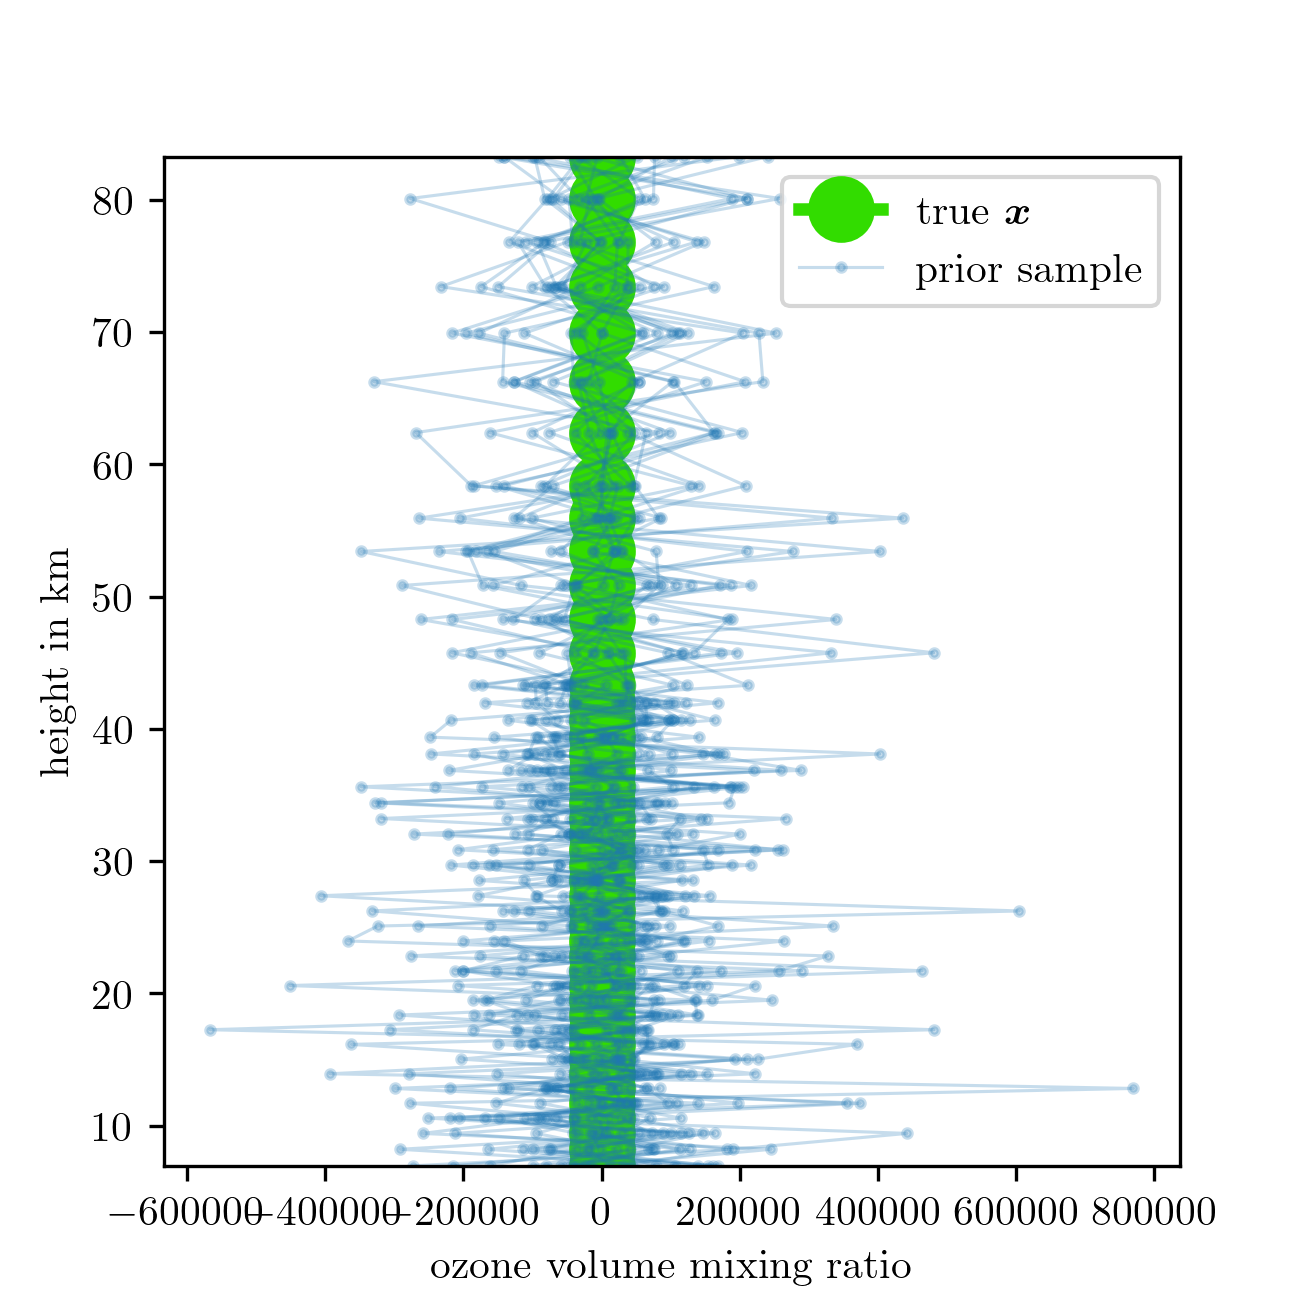
\includegraphics{OzonePrior.png}
	\caption[Samples from ozone prior distribution.]{We draw samples from ozone prior distribution $\bm{x} \sim \mathcal{N}(0,\delta \bm{L})$ after generating a sample from the hyper-prior distribution $\delta \sim \mathcal{T}(1,10^{-10})$. Note that since the variance of prior samples is very large compared to the ozone volume mixing ratios, the ozone profile appears to be constant, which is not the case, see e.g. Fig. \ref{fig:O3Samp}.}
	\label{fig:O3Prior}
\end{figure}


\subsection{Integrated Autocorrelation plots} 

\begin{figure}[ht!]
	\centering
	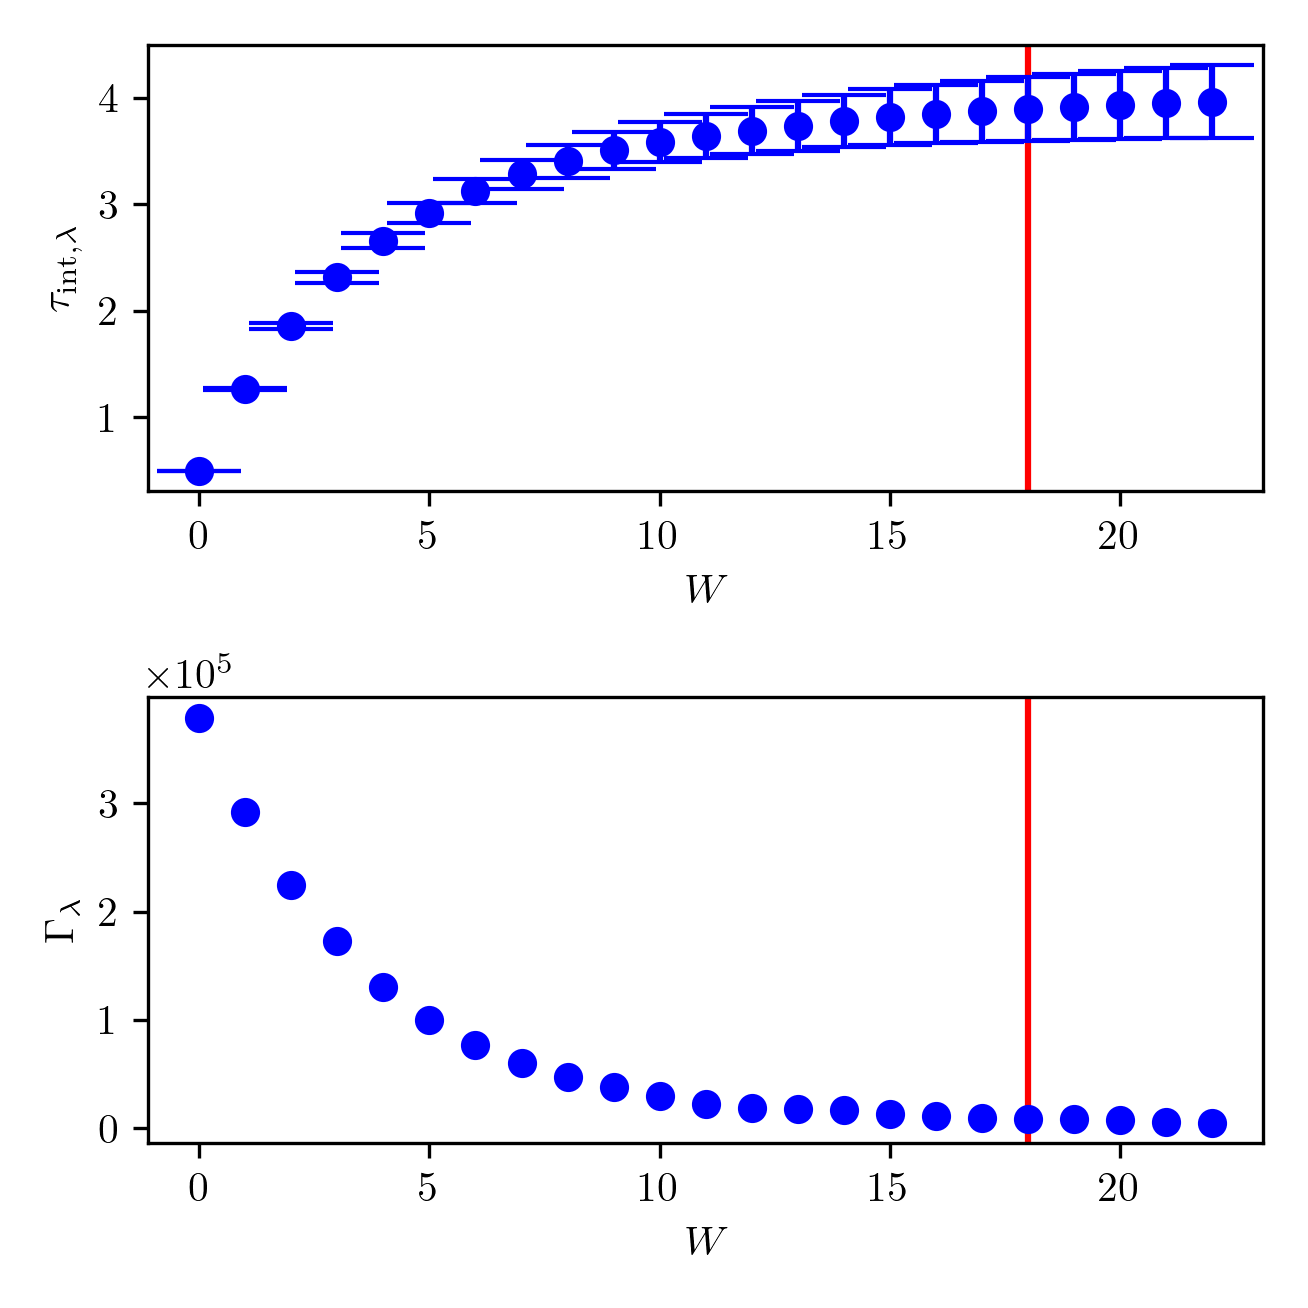
\includegraphics{UwerrTauIntSecO3lam.png}
	\caption[IACT and autocorrelation function for samples $\lambda \sim \pi{\cdot | \gamma, \bm{y}}$.]{IACT for samples $\lambda \sim \pi( \cdot | \gamma, \bm{y})$ based on the approximated forward model.}
	\label{fig:}
\end{figure}
\begin{figure}[ht!]
	\centering
	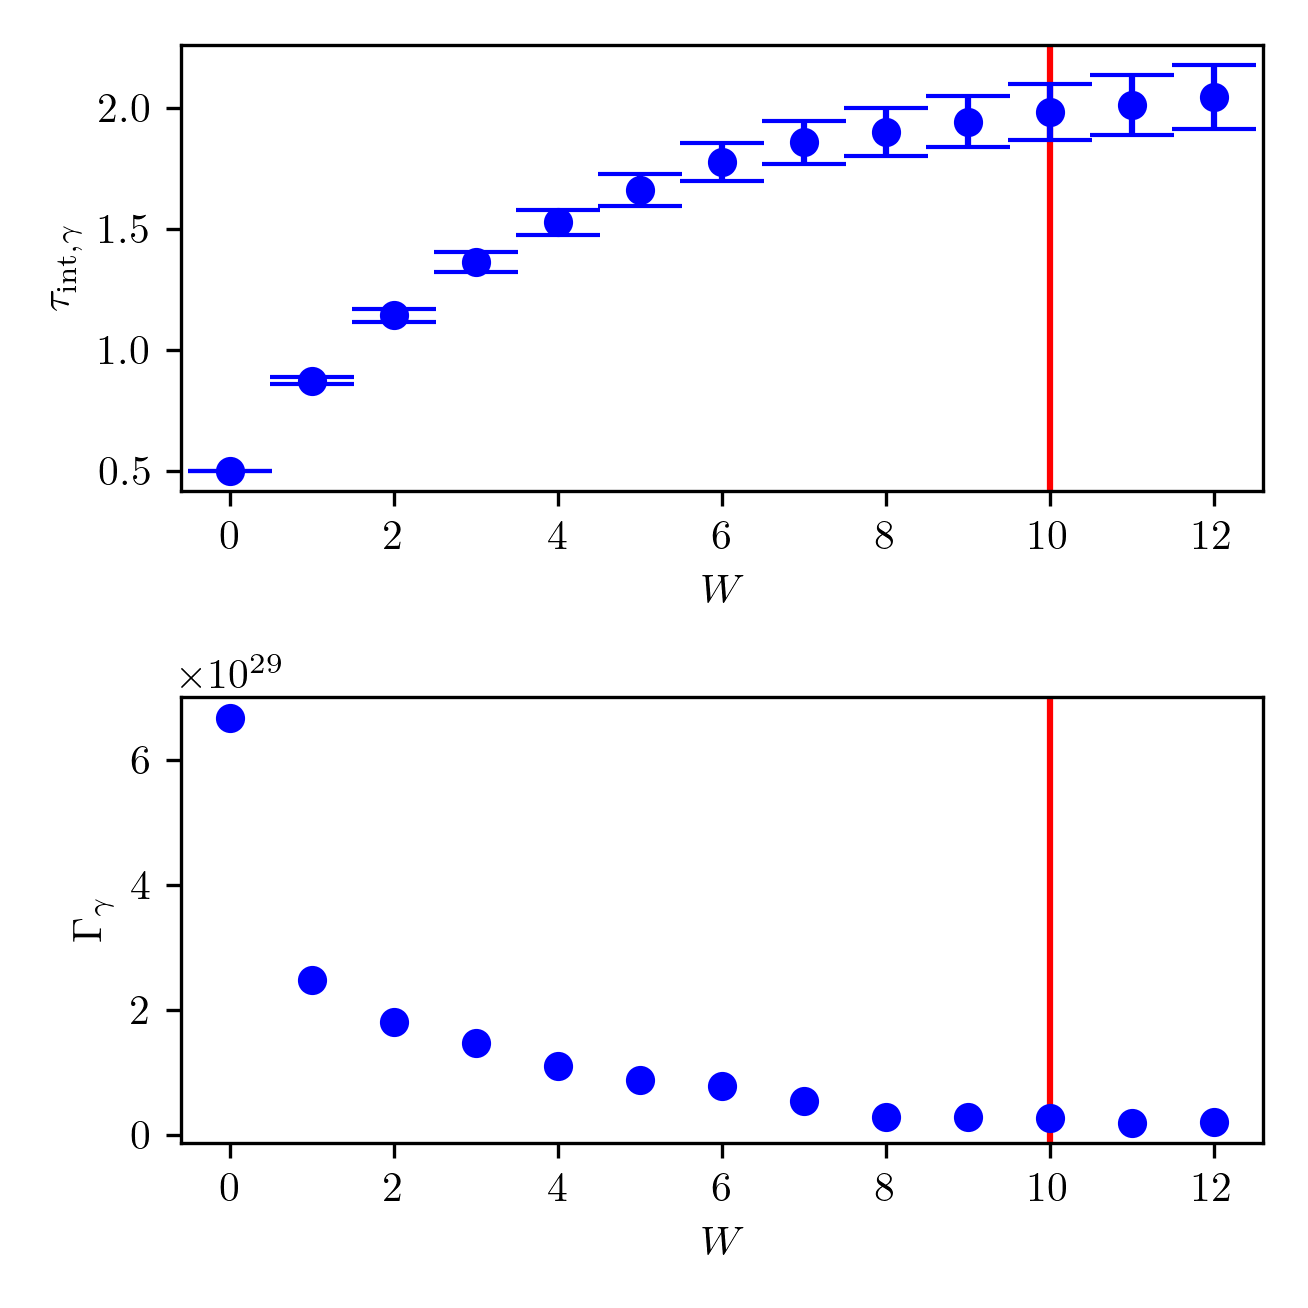
\includegraphics{UwerrTauIntSecO3gam.png}
	\caption[IACT and autocorrelation function for samples $\gamma \sim \pi( \cdot | \lambda, \bm{y})$]{IACT for samples $\gamma \sim \pi( \cdot | \lambda, \bm{y})$ based on the approximated forward model.}
	\label{fig:}
\end{figure}
\clearpage
\section{Pressure and Temperature}

\subsection{Priors}
\begin{figure}[ht!]
	\centering
	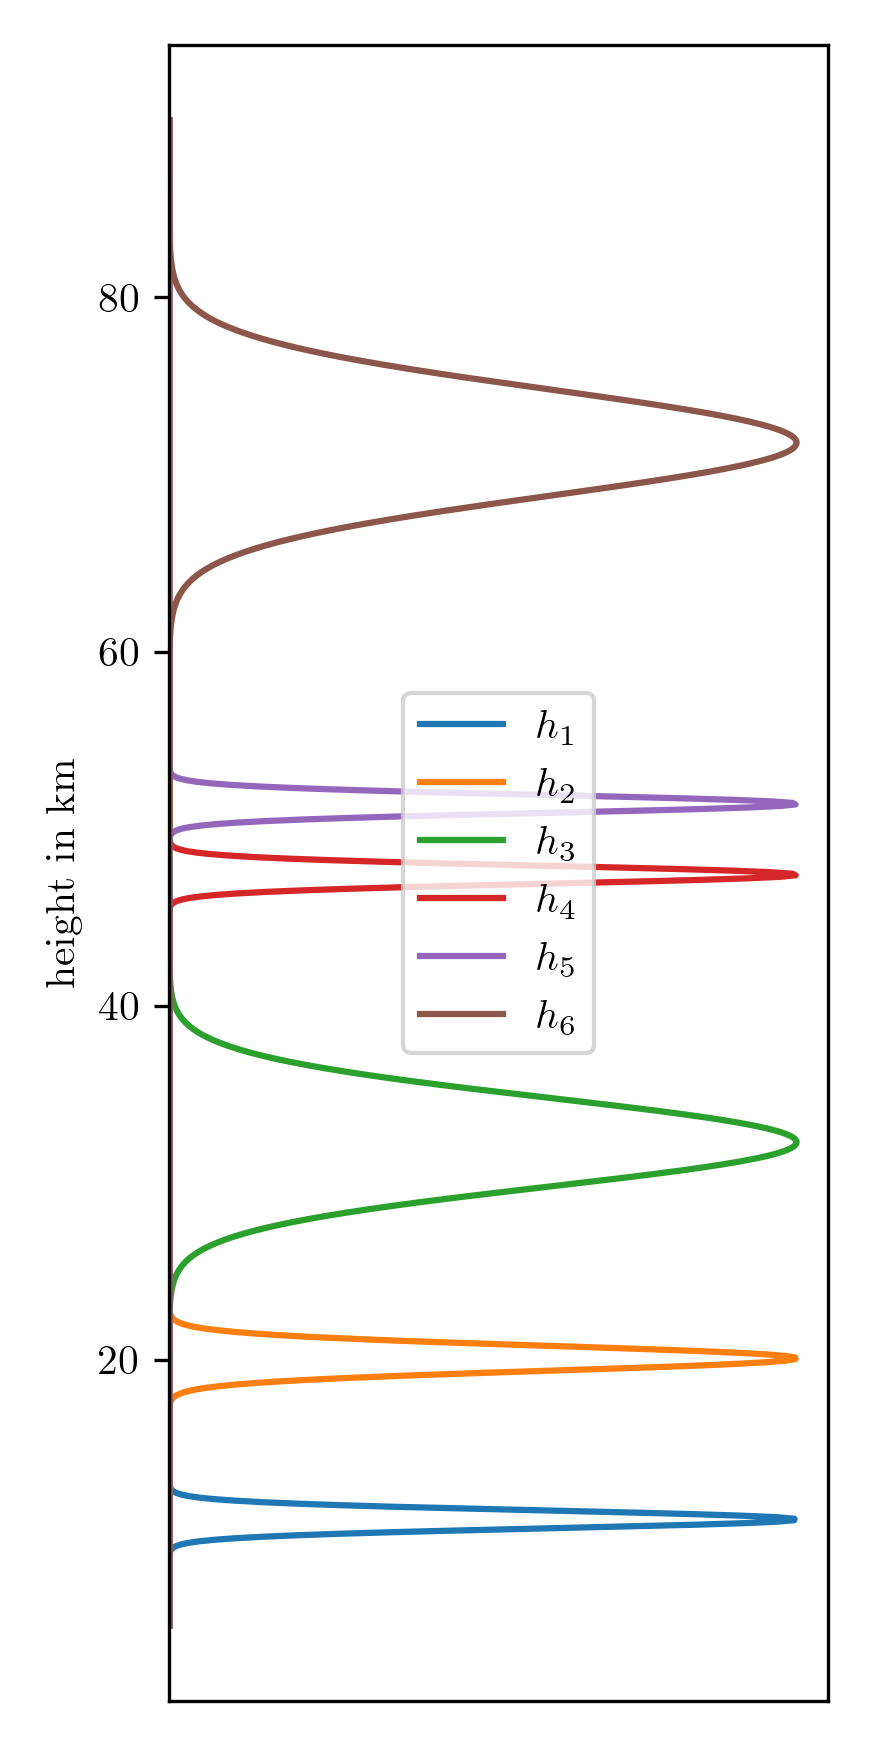
\includegraphics{HeightPriors.png}
	\caption[Prior distributions $\pi(\bm{h_T})$.]{Prior distributions $\pi(\bm{h_T})$, which we choose so that they do not overlap and not conflict with the temperature function \ref{eq:tempFunc}}
	\label{fig:HeightPriors}
\end{figure} 

\begin{figure}[ht!]
	\centering
	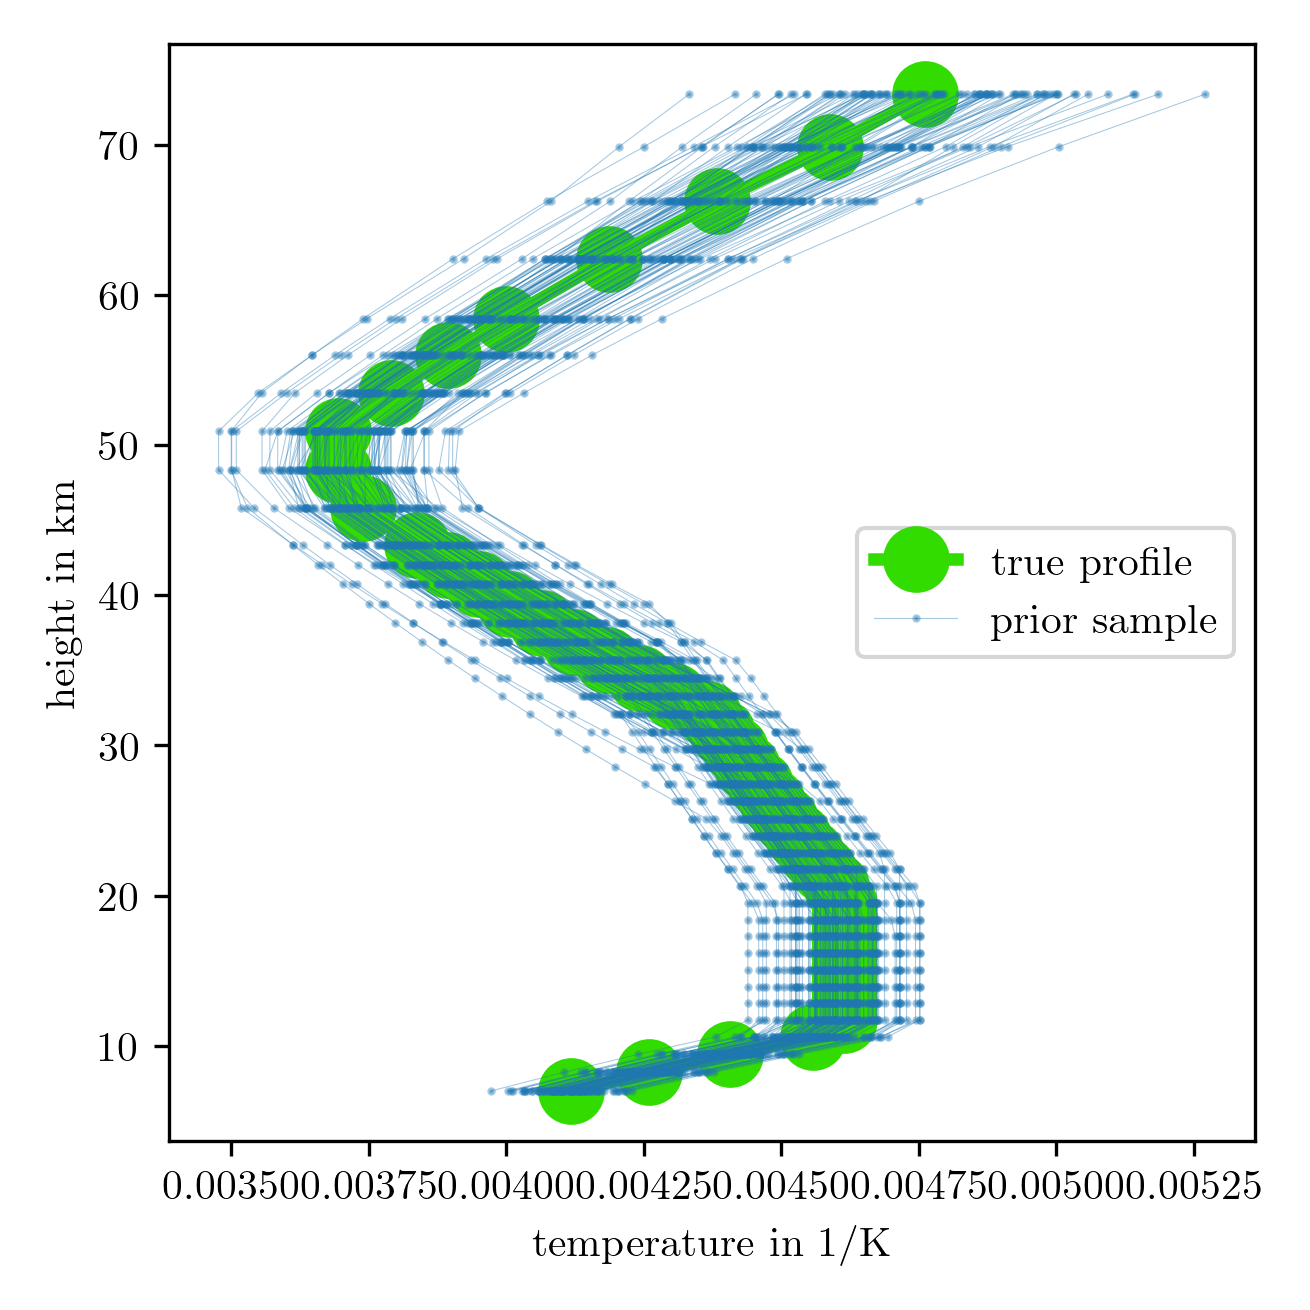
\includegraphics{PriorOverTempPost.png}
	\caption[Prior samples of $1/\bm{T}$]{Prior samples of the inverted temperature profile.}
	\label{fig:OverTempPrior}
\end{figure}
\subsection{T-walk Trace}
\begin{figure}[ht!]
	\centering
	\includegraphics{TraceTwalk.png}
	\caption[T-walk trace]{Output trace of the t-walk on the posterior distribution $\pi(p_0,b,\bm{h_T},\bm{a}| \gamma,\bm{y})$.}
	\label{fig:TraceTwalk}
\end{figure}

\subsection{Integrated Autocorrelation Plots} 
\begin{figure}[ht!]
	\centering
	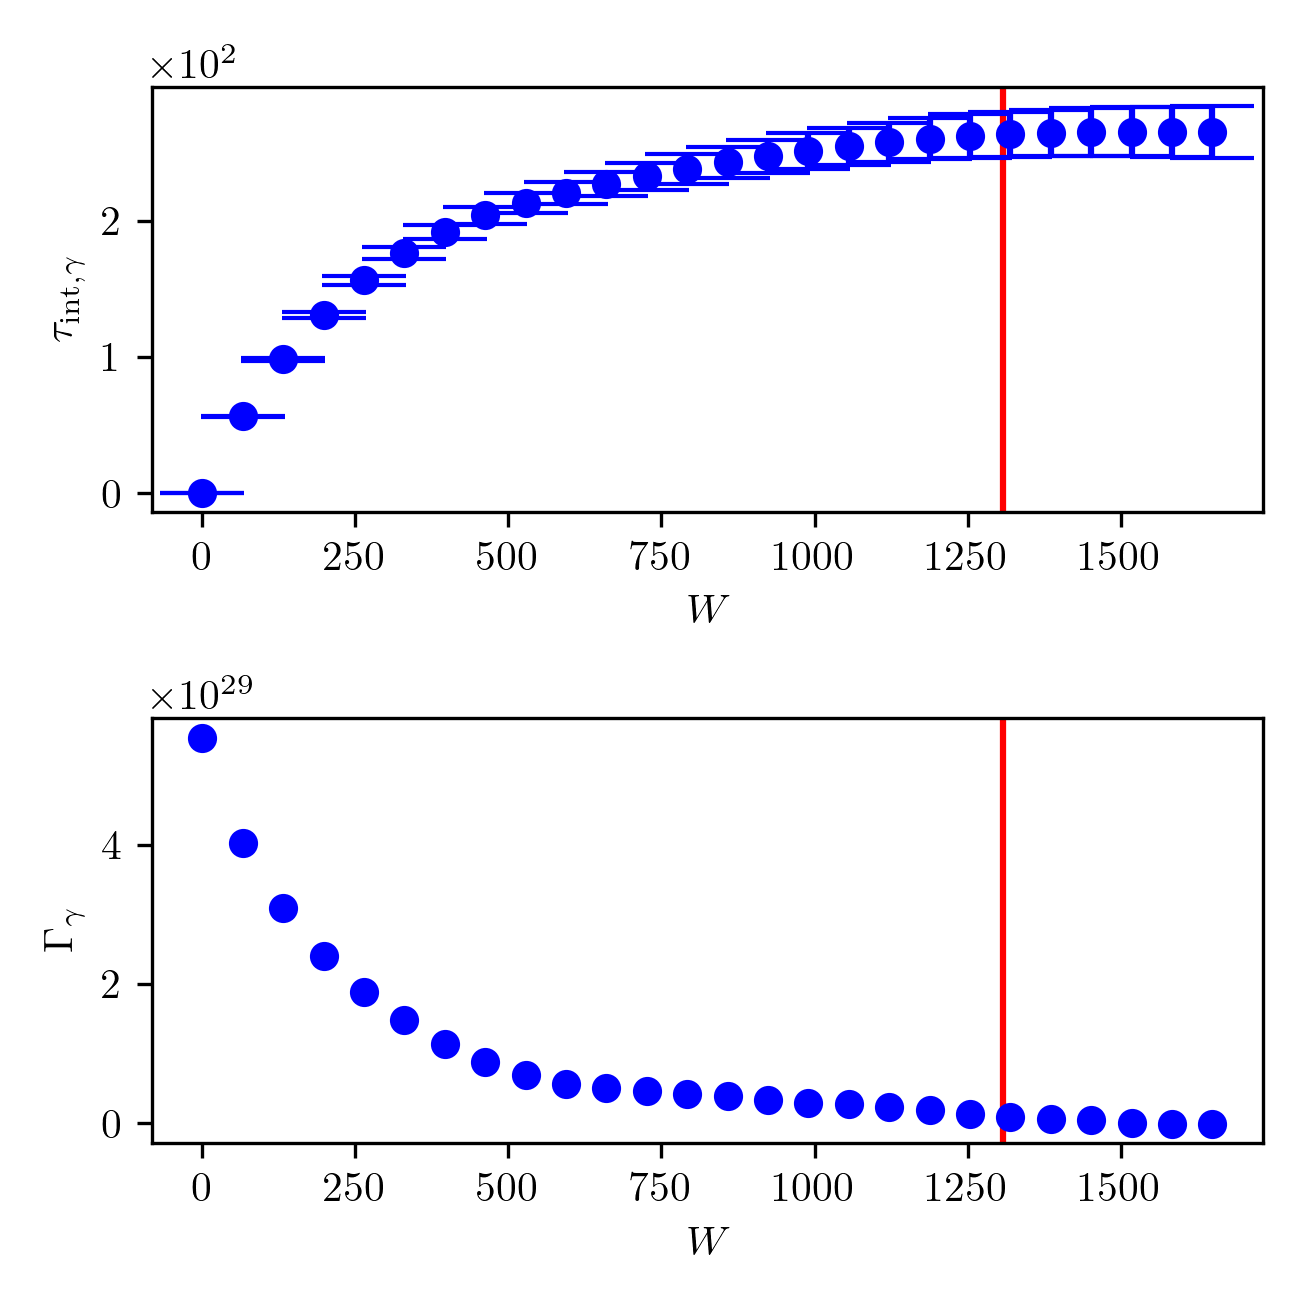
\includegraphics{UwerrTauIntTWalk0.png}
	\caption[IACT and autocorrelation function for $h_{T,1}$ samples.]{IACT and autocorrelation function for samples $h_1 \sim \pi( \cdot |h_{T,2},h_{T,3},h_{T,4},h_{T,5},h_{T,6},a_0,a_1,a_2,a_3,a_4,a_5,a_6,T_0,b,p_0, \bm{y})$}
	\label{fig:}
\end{figure}
\begin{figure}[ht!]
	\centering
	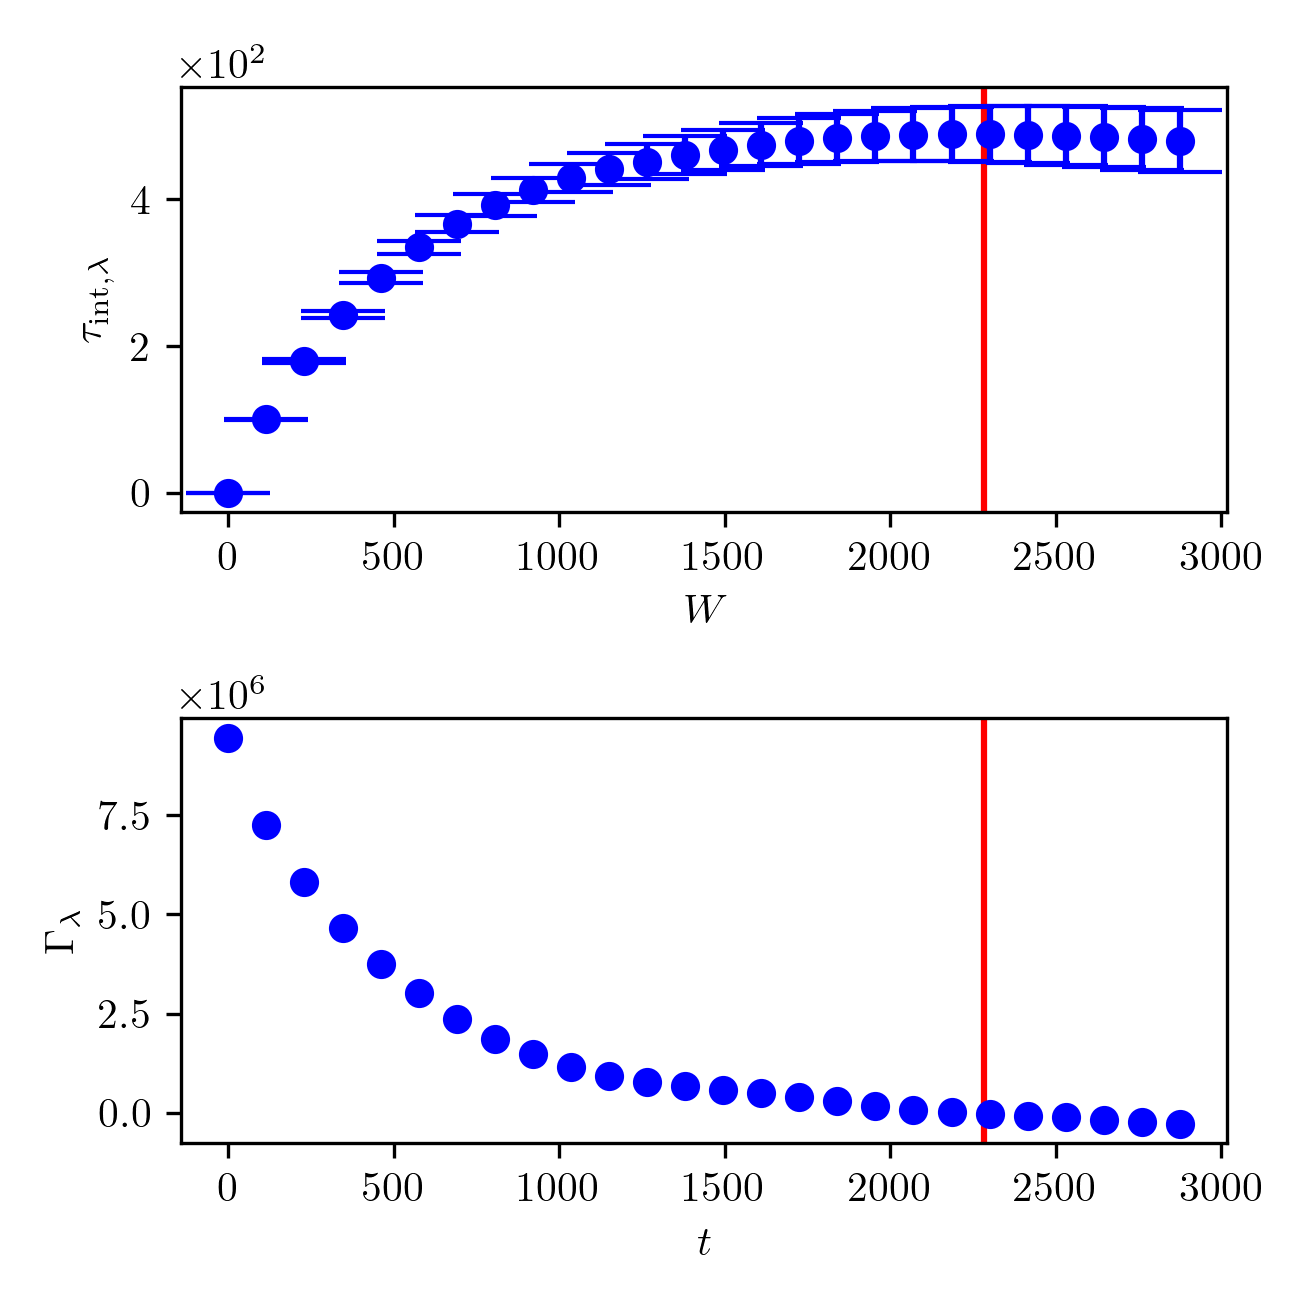
\includegraphics{UwerrTauIntTWalk1.png}
	\caption[IACT and autocorrelation function for $h_2$ samples.]{IACT and autocorrelation function for samples $h_2 \sim \pi( \cdot | h_1,h_3,h_4,h_5,h_6,a_0,a_1,a_2,a_3,a_4,a_5,a_6,T_0,b,p_0, \bm{y})$}
	\label{fig:}
\end{figure}


\begin{figure}[ht!]
	\centering
	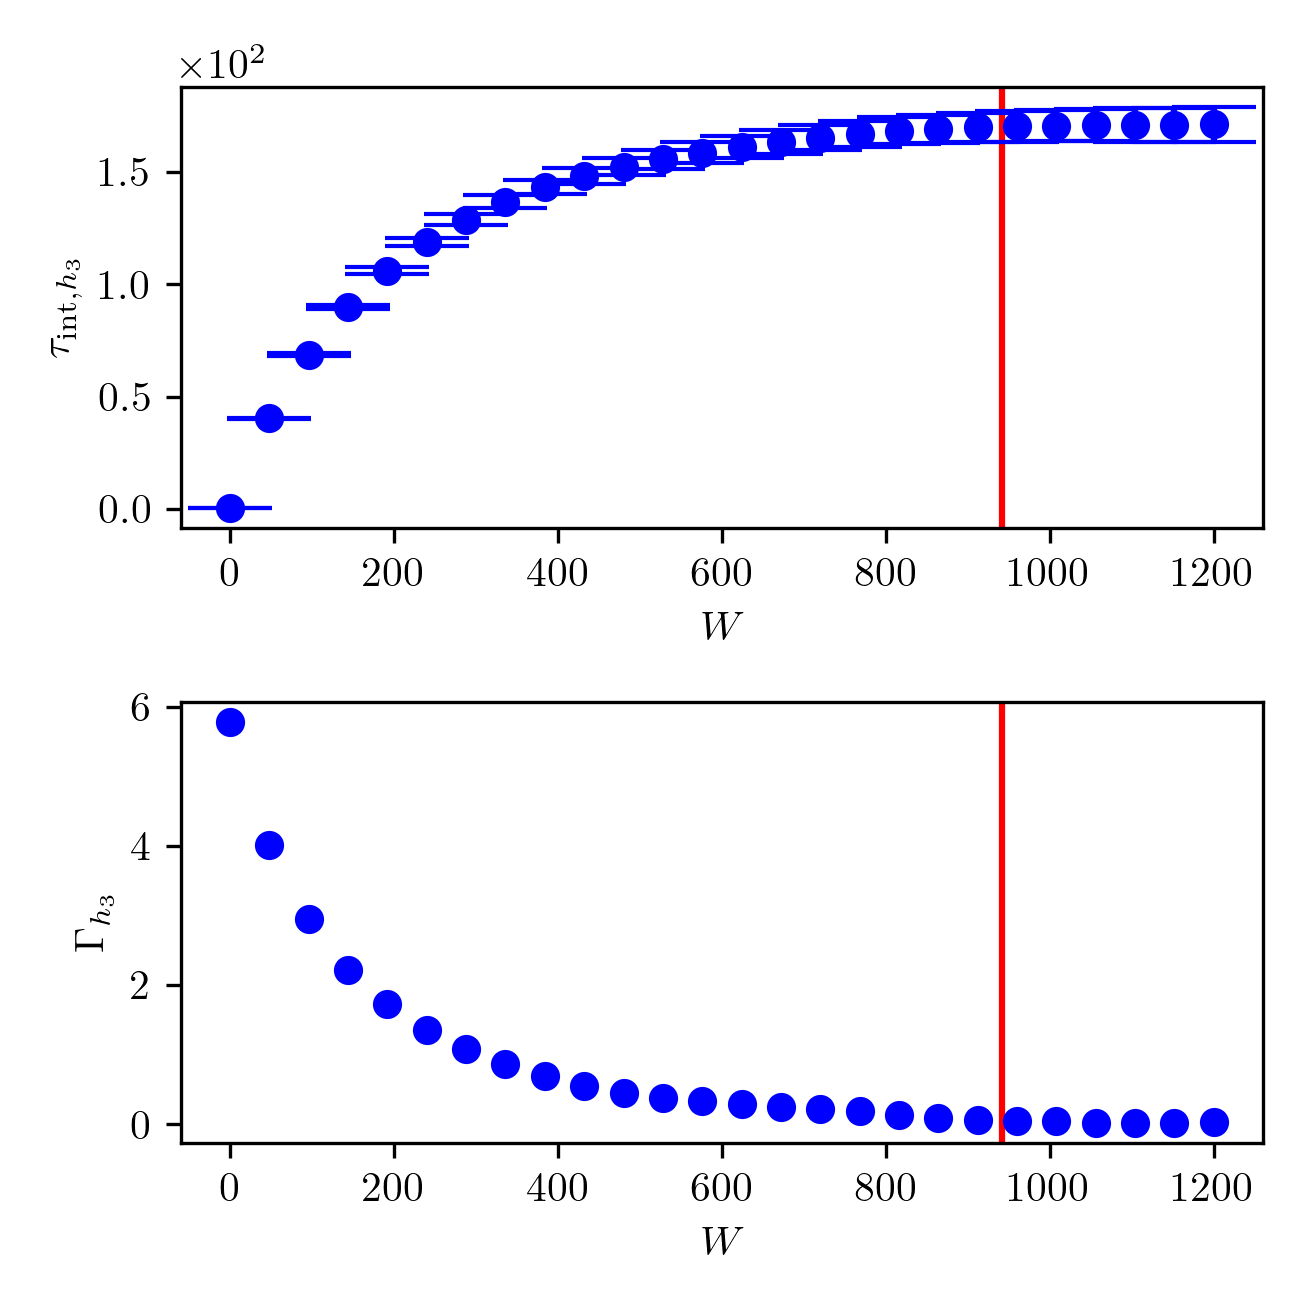
\includegraphics{UwerrTauIntTWalk2.png}
	\caption[IACT and autocorrelation function for $h_3$ samples.]{IACT and autocorrelation function for samples $h_3 \sim \pi( \cdot | h_1,h_2,h_4,h_5,h_6,a_0,a_1,a_2,a_3,a_4,a_5,a_6,T_0,b,p_0, \bm{y})$}
	\label{fig:}
\end{figure}


\begin{figure}[ht!]
	\centering
	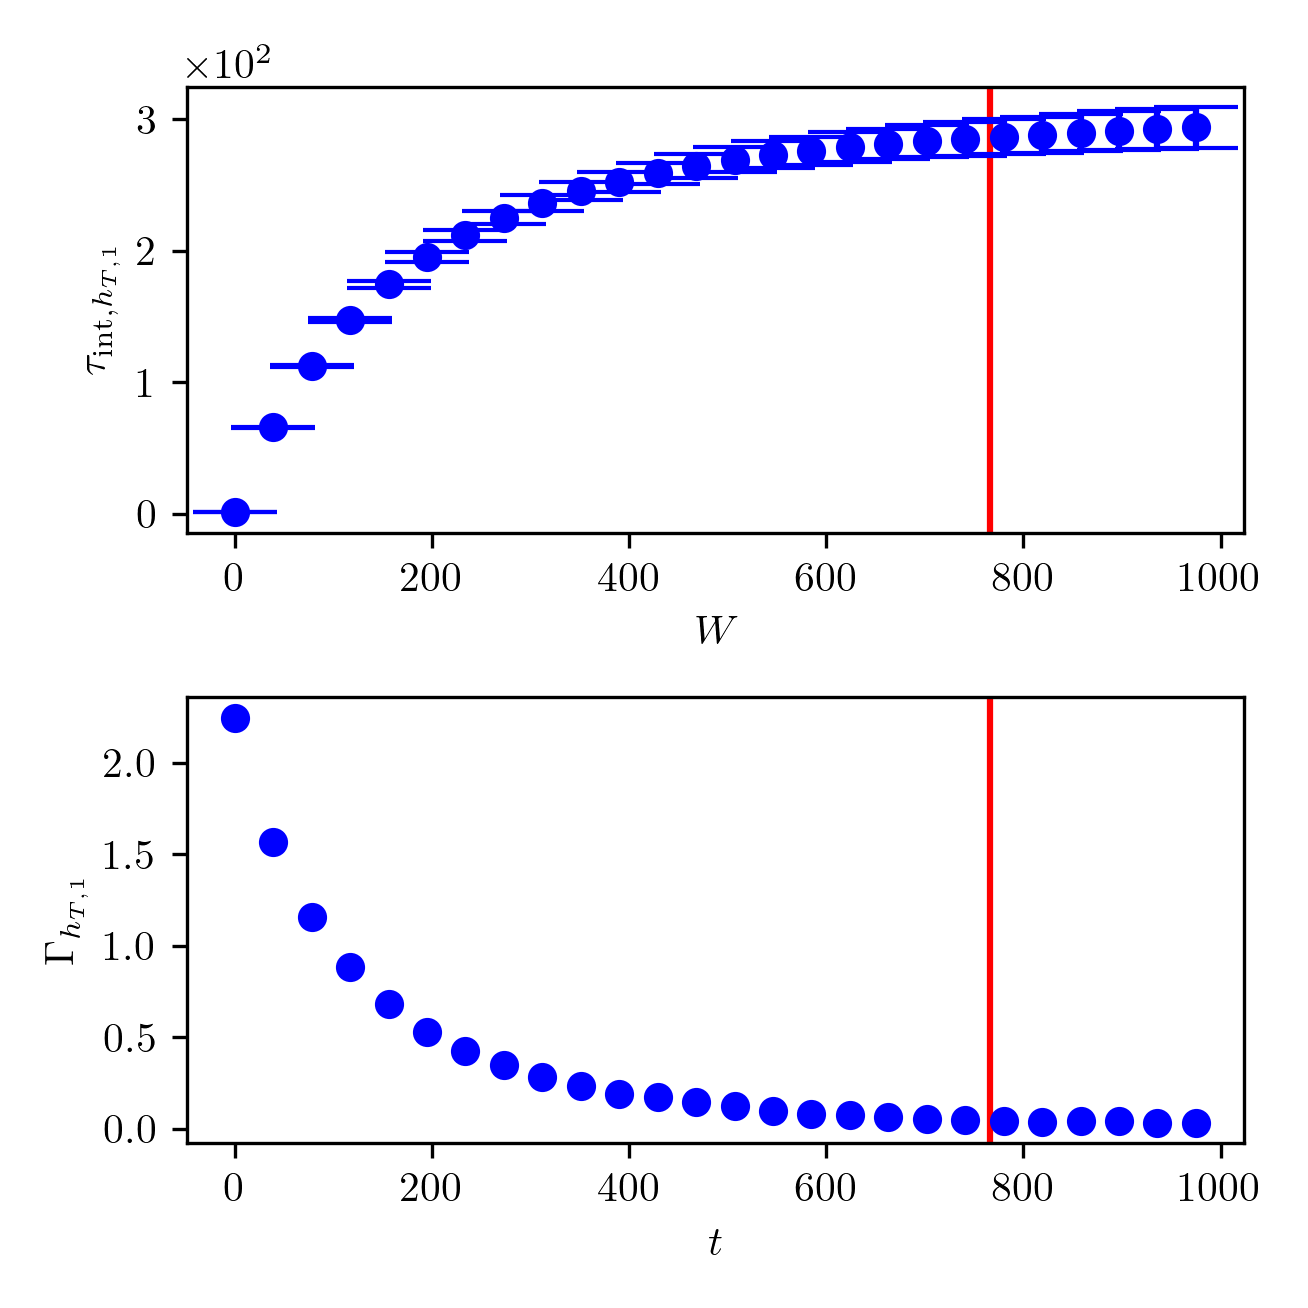
\includegraphics{UwerrTauIntTWalk3.png}
	\caption[IACT and autocorrelation function for $h_4$ samples.]{IACT and autocorrelation function for samples $h_4 \sim \pi( \cdot | h_1,h_2,h_3,h_5,h_6,a_0,a_1,a_2,a_3,a_4,a_5,a_6,T_0,b,p_0, \bm{y})$}
	\label{fig:}
\end{figure}


\begin{figure}[ht!]
	\centering
	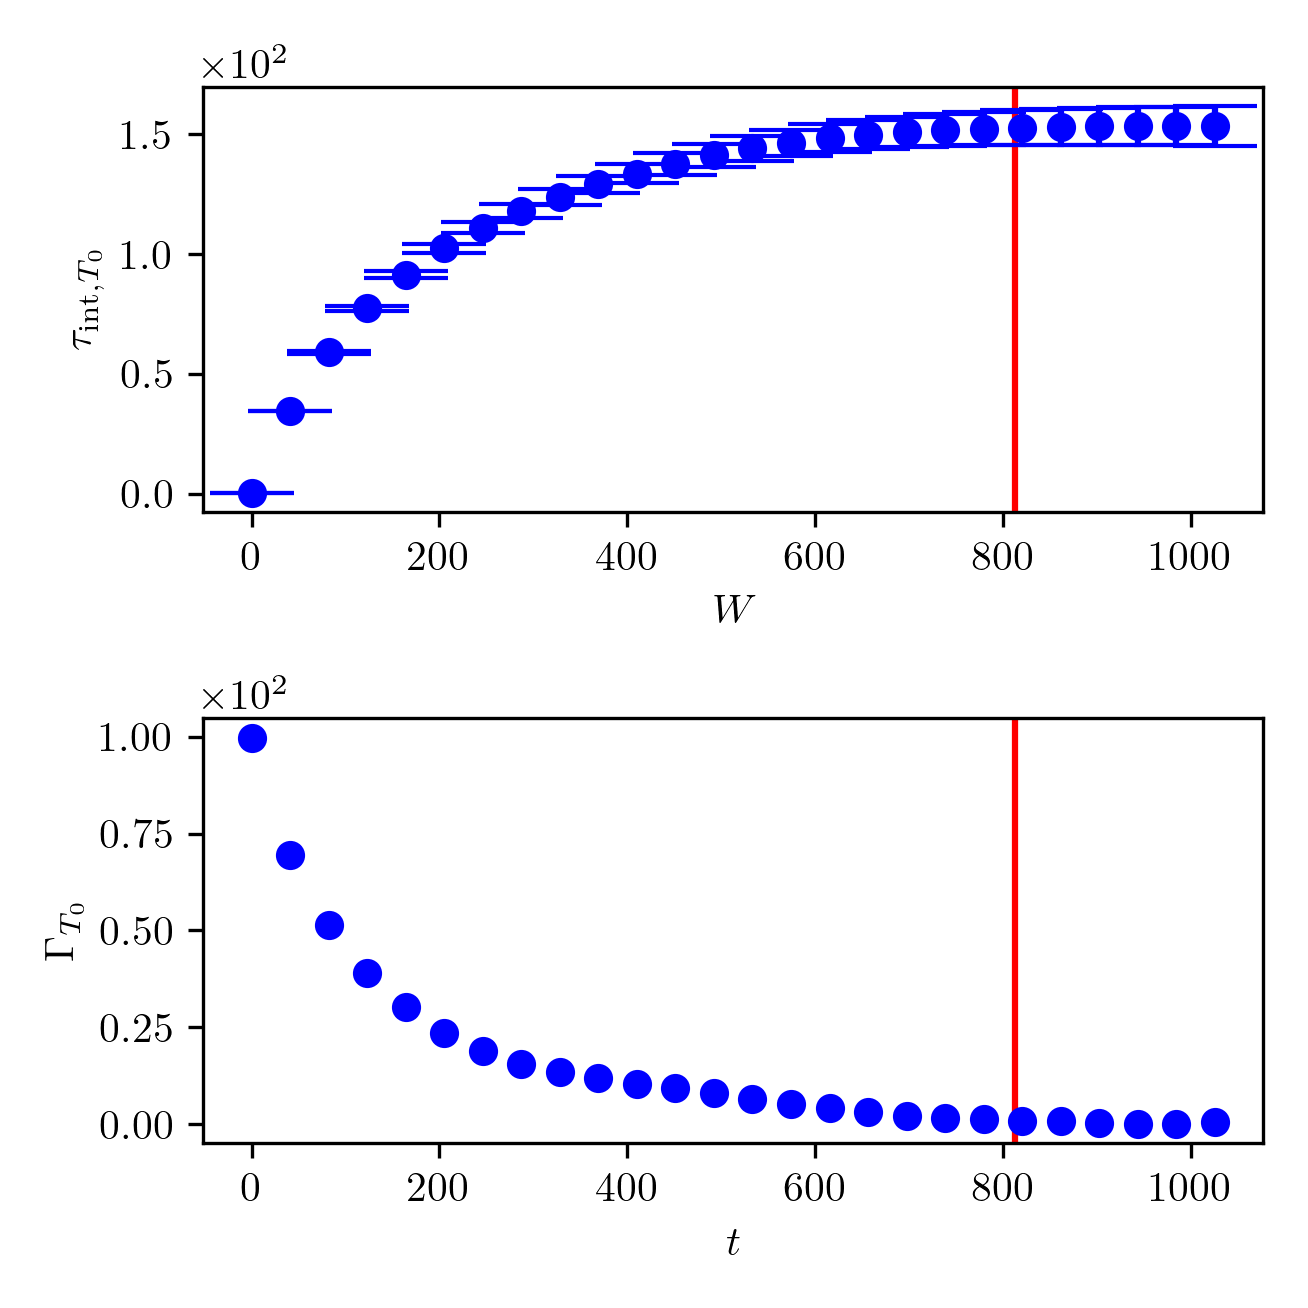
\includegraphics{UwerrTauIntTWalk4.png}
	\caption[IACT and autocorrelation function for $h_5$ samples.]{IACT and autocorrelation function for samples $h_5 \sim \pi( \cdot | h_1, h_2,h_3,h_4,h_6,a_0,a_1,a_2,a_3,a_4,a_5,a_6,T_0,b,p_0,  \bm{y})$}
	\label{fig:}
\end{figure}


\begin{figure}[ht!]
	\centering
	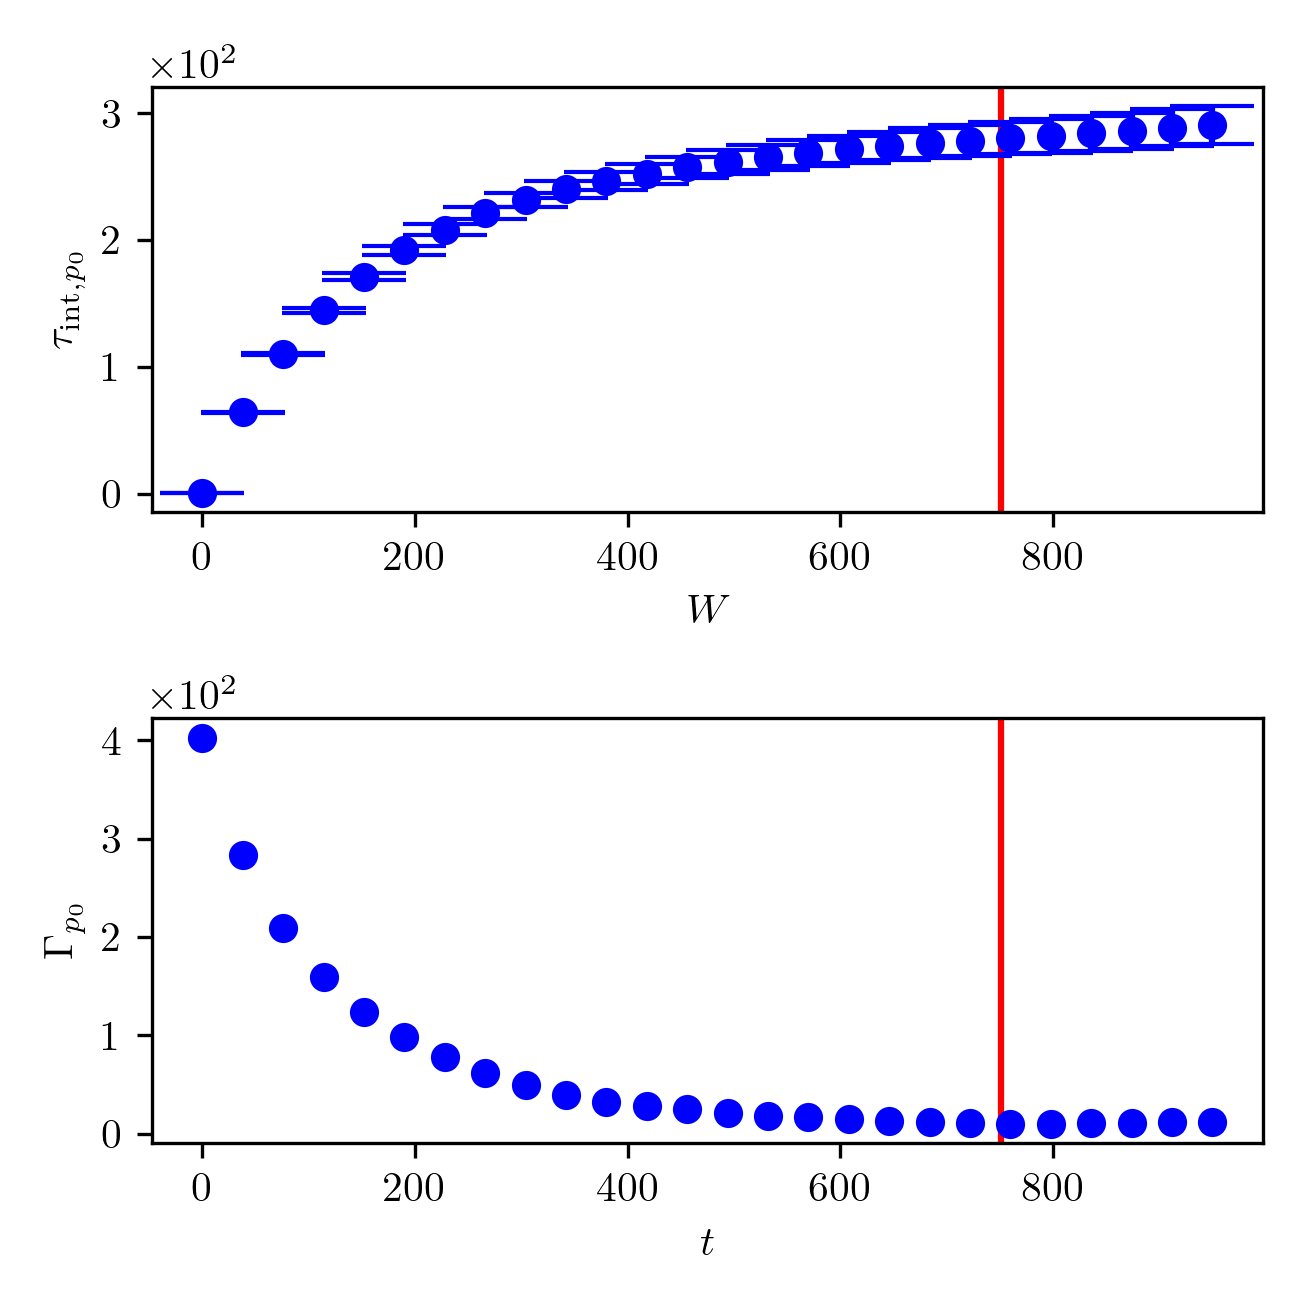
\includegraphics{UwerrTauIntTWalk5.png}
	\caption[IACT and autocorrelation function for $h_6$ samples.]{IACT and autocorrelation function for samples $h_6 \sim \pi( \cdot | h_1, h_2,h_3,h_4,h_5,a_0,a_1,a_2,a_3,a_4,a_5,a_6,T_0,b,p_0,  \bm{y})$}
	\label{fig:}
\end{figure}


\begin{figure}[ht!]
	\centering
	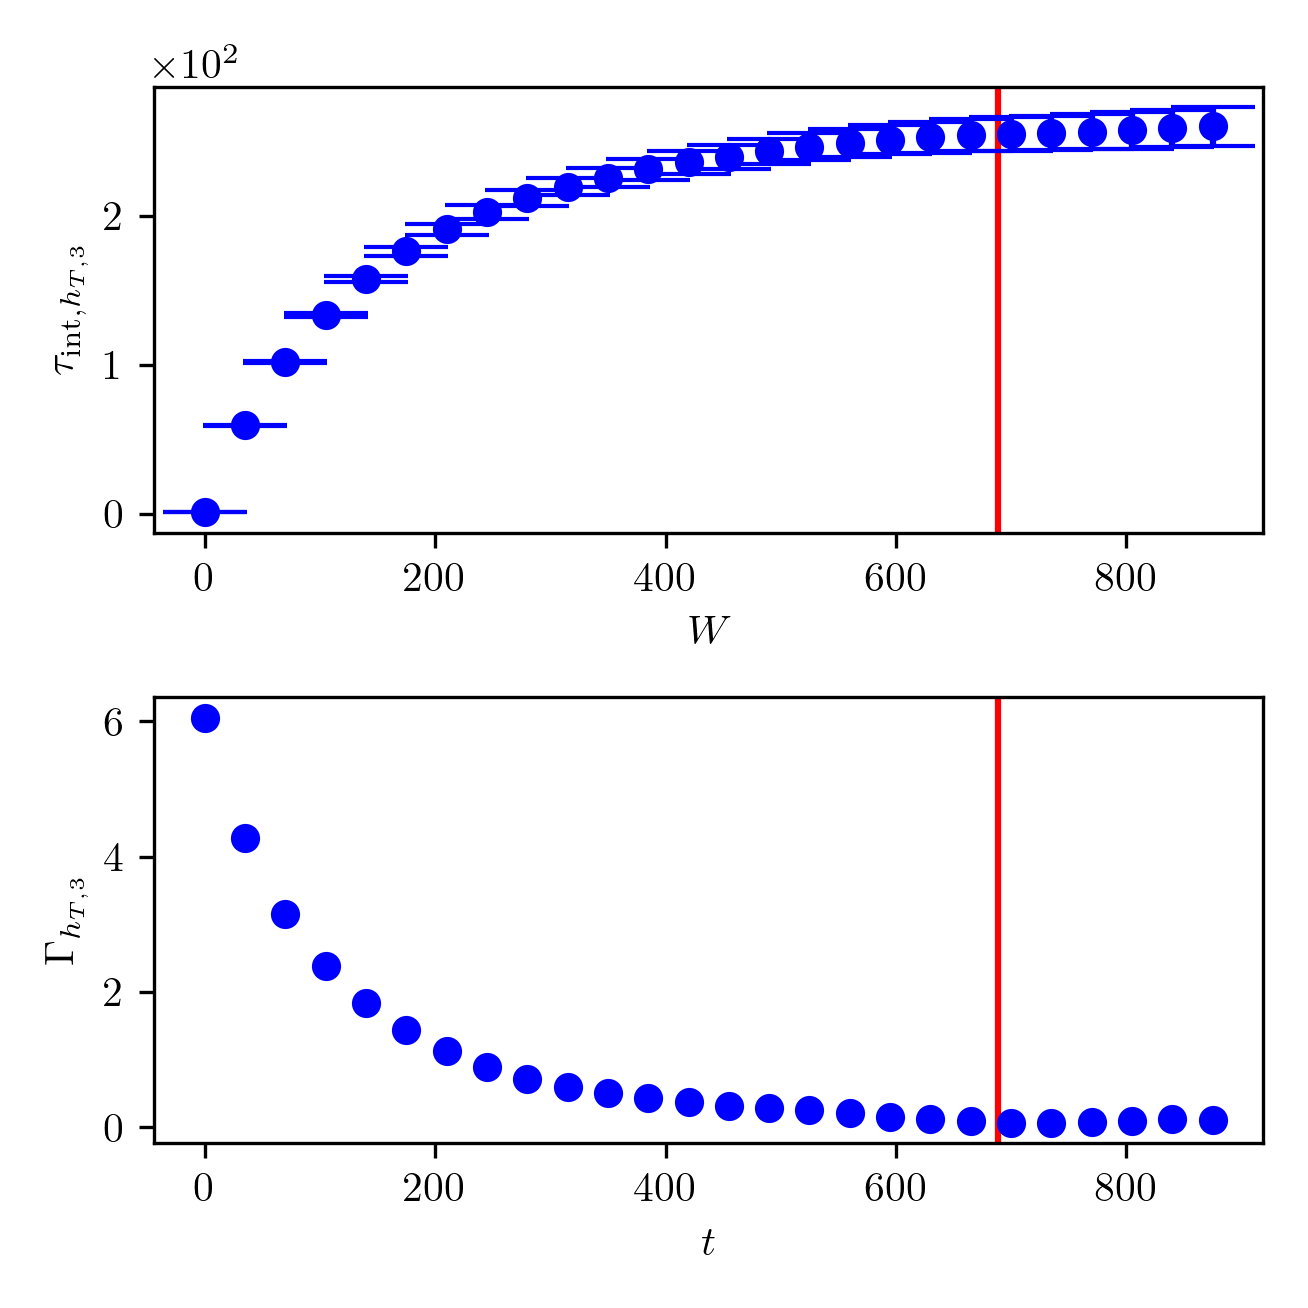
\includegraphics{UwerrTauIntTWalk6.png}
	\caption[IACT and autocorrelation function for $a_0$ samples.]{IACT and autocorrelation function for samples $a_0 \sim \pi( \cdot | h_1, h_2,h_3,h_4,h_5,h_6,a_1,a_2,a_3,a_4,a_5,a_6,T_0,b,p_0,  \bm{y})$}
	\label{fig:}
\end{figure}

\begin{figure}[ht!]
	\centering
	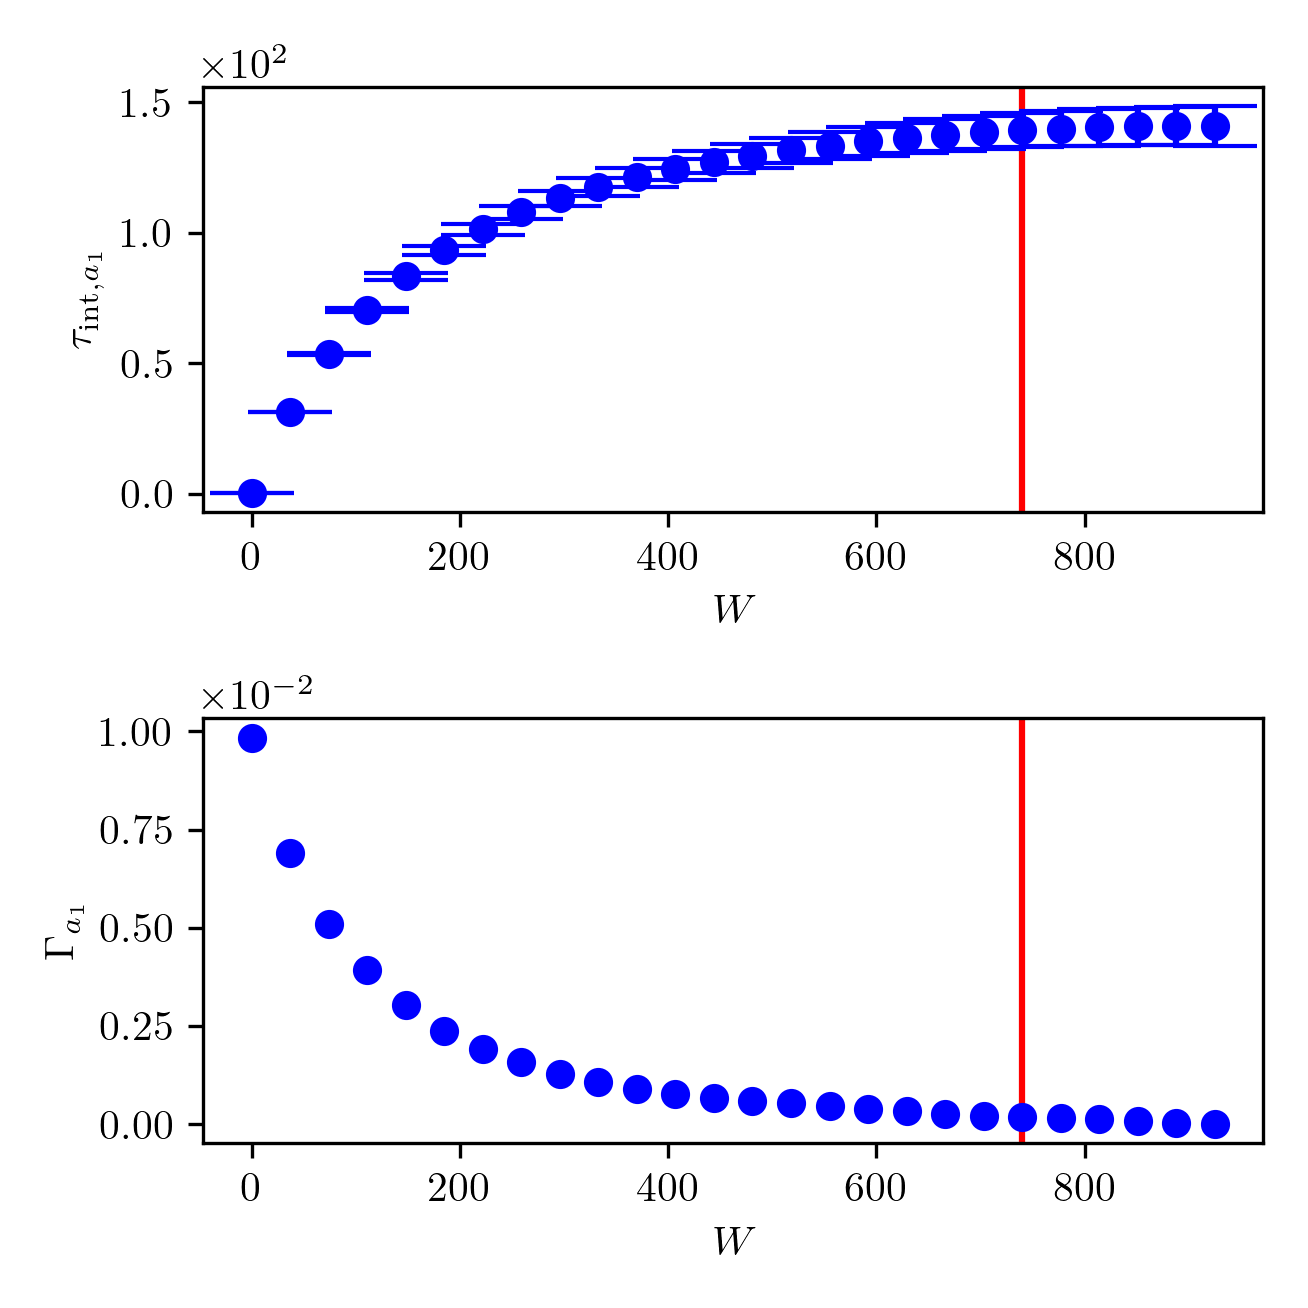
\includegraphics{UwerrTauIntTWalk7.png}
	\caption[IACT and autocorrelation function for $a_1$ samples.]{IACT and autocorrelation function for samples $a_1 \sim \pi( \cdot | h_1, h_2,h_3,h_4,h_5,h_6,a_0,a_2,a_3,a_4,a_5,a_6,T_0,b,p_0,  \bm{y})$}
	\label{fig:}
\end{figure}


\begin{figure}[ht!]
	\centering
	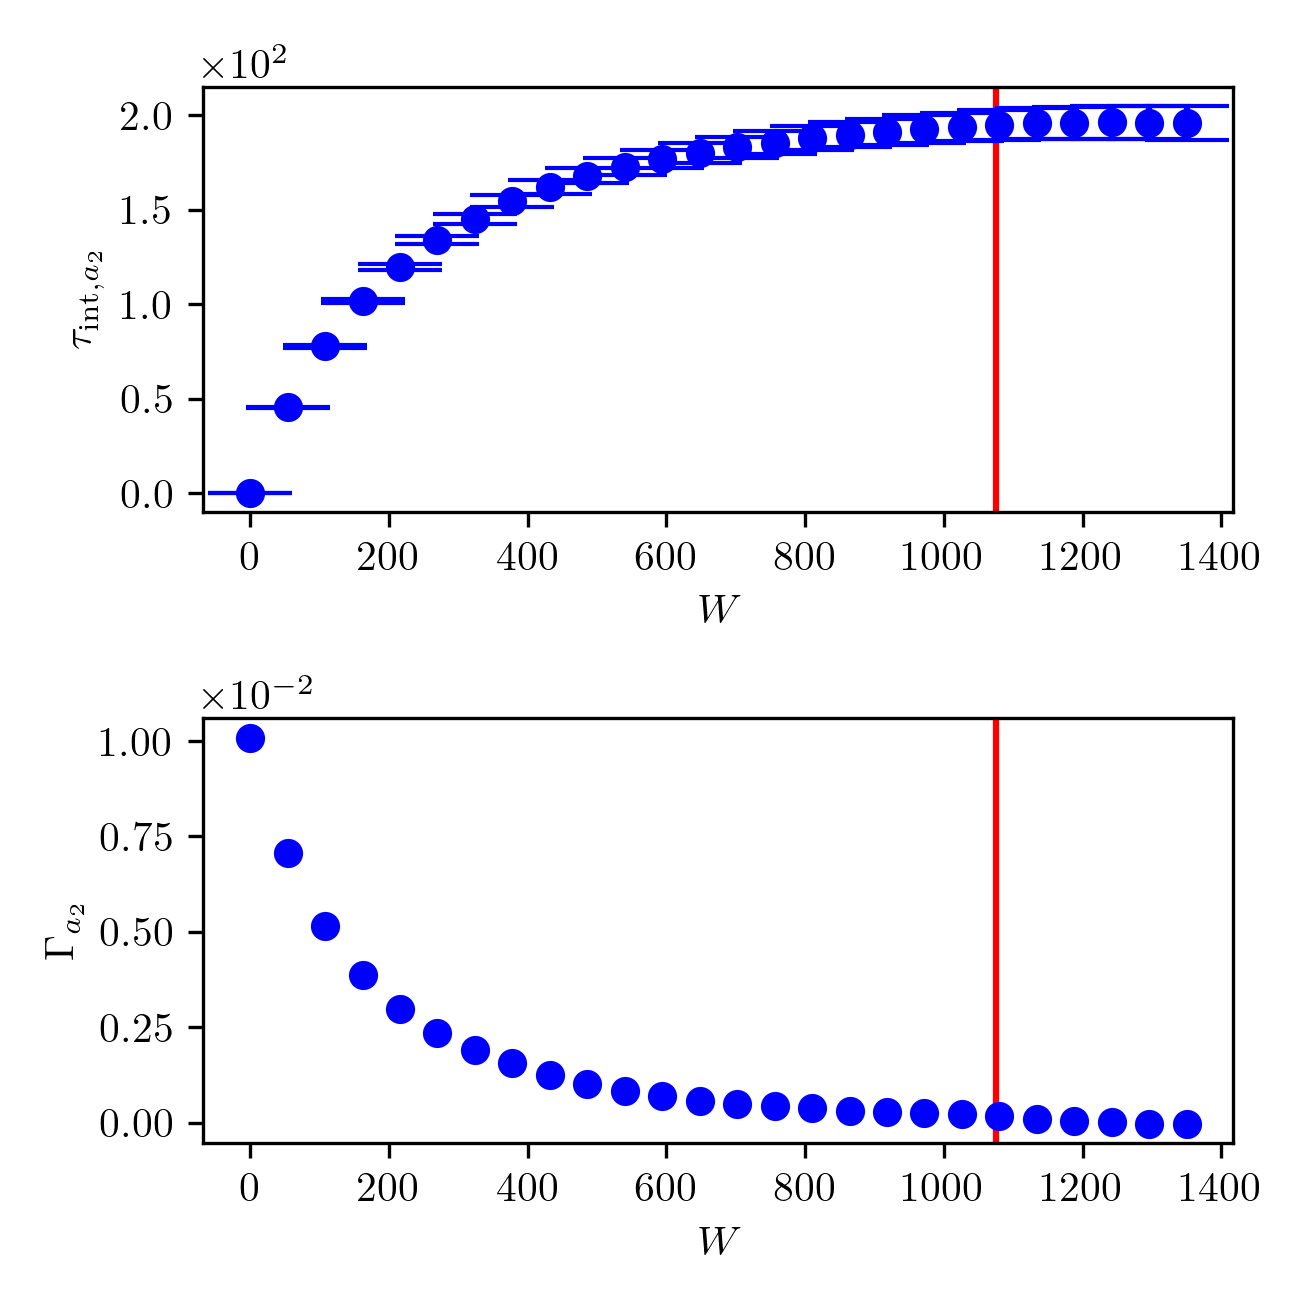
\includegraphics{UwerrTauIntTWalk8.png}
	\caption[IACT and autocorrelation function for $a_2$ samples.]{IACT and autocorrelation function for samples $a_2 \sim \pi( \cdot | h_1, h_2,h_3,h_4,h_5,h_6,a_0,a_1,a_3,a_4,a_5,a_6,T_0,b,p_0,  \bm{y})$}
	\label{fig:}
\end{figure}


\begin{figure}[ht!]
	\centering
	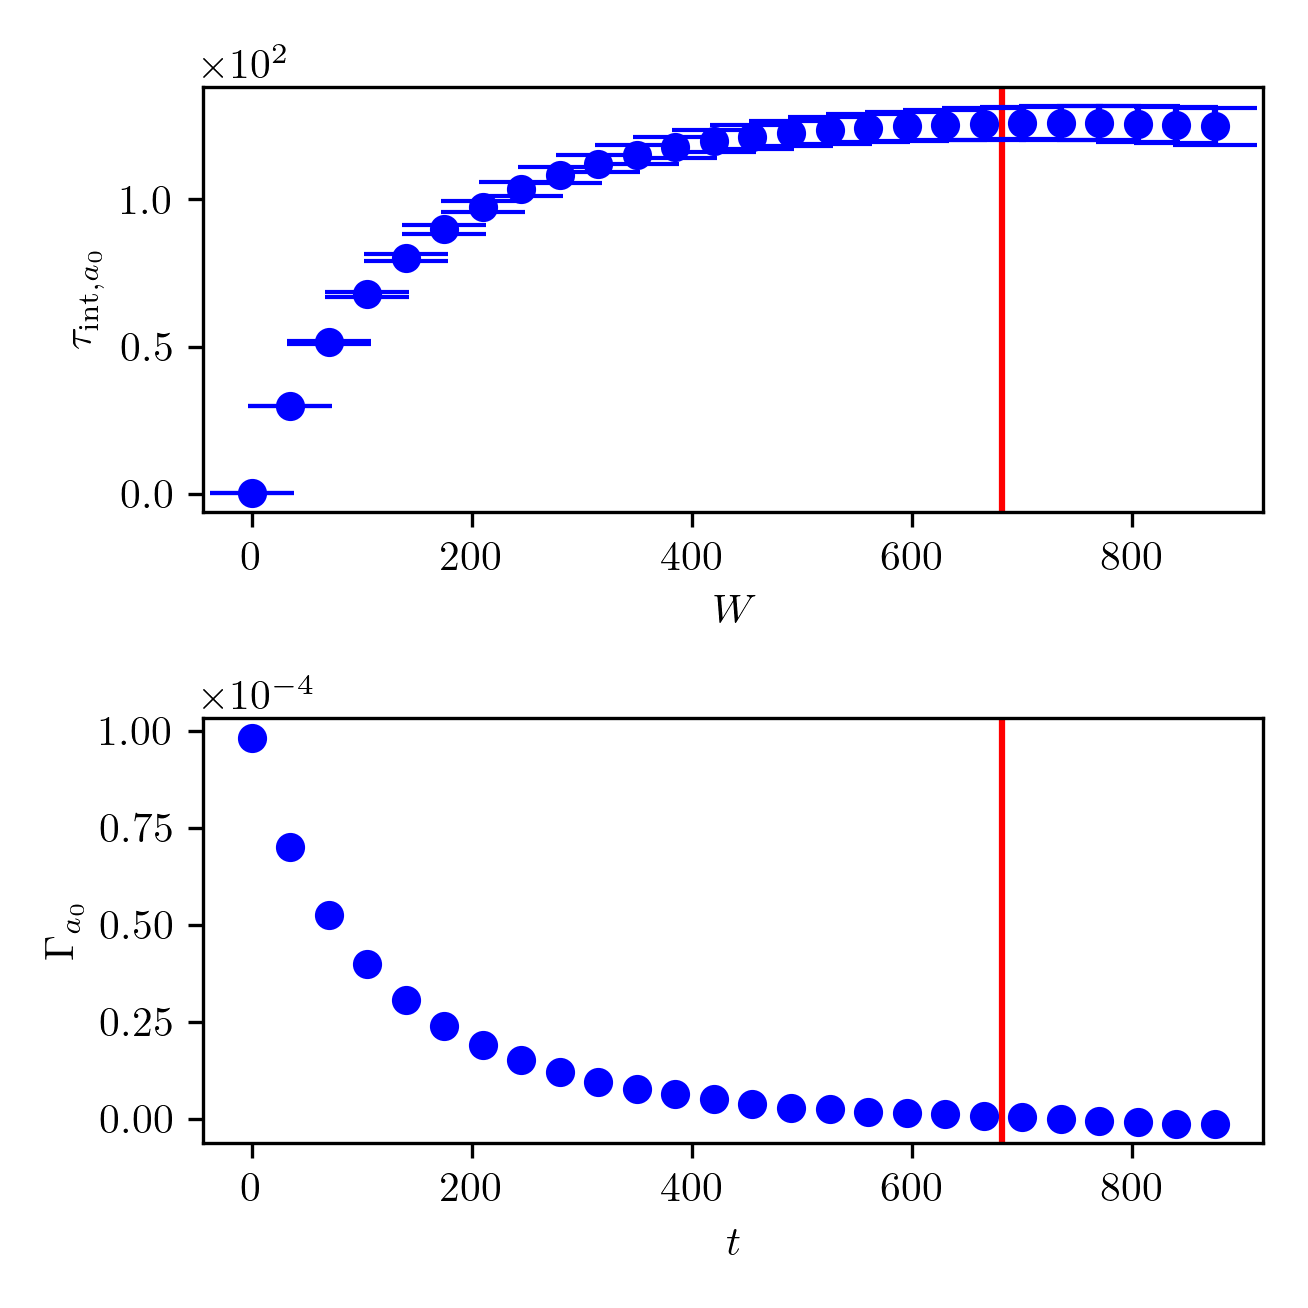
\includegraphics{UwerrTauIntTWalk9.png}
	\caption[IACT and autocorrelation function for $a_3$ samples.]{IACT and autocorrelation function for samples $a_3 \sim \pi( \cdot | h_1, h_2,h_3,h_4,h_5,h_6,a_0,a_1,a_2,a_4,a_5,a_6,T_0,b,p_0,  \bm{y})$}
	\label{fig:}
\end{figure}

\begin{figure}[ht!]
	\centering
	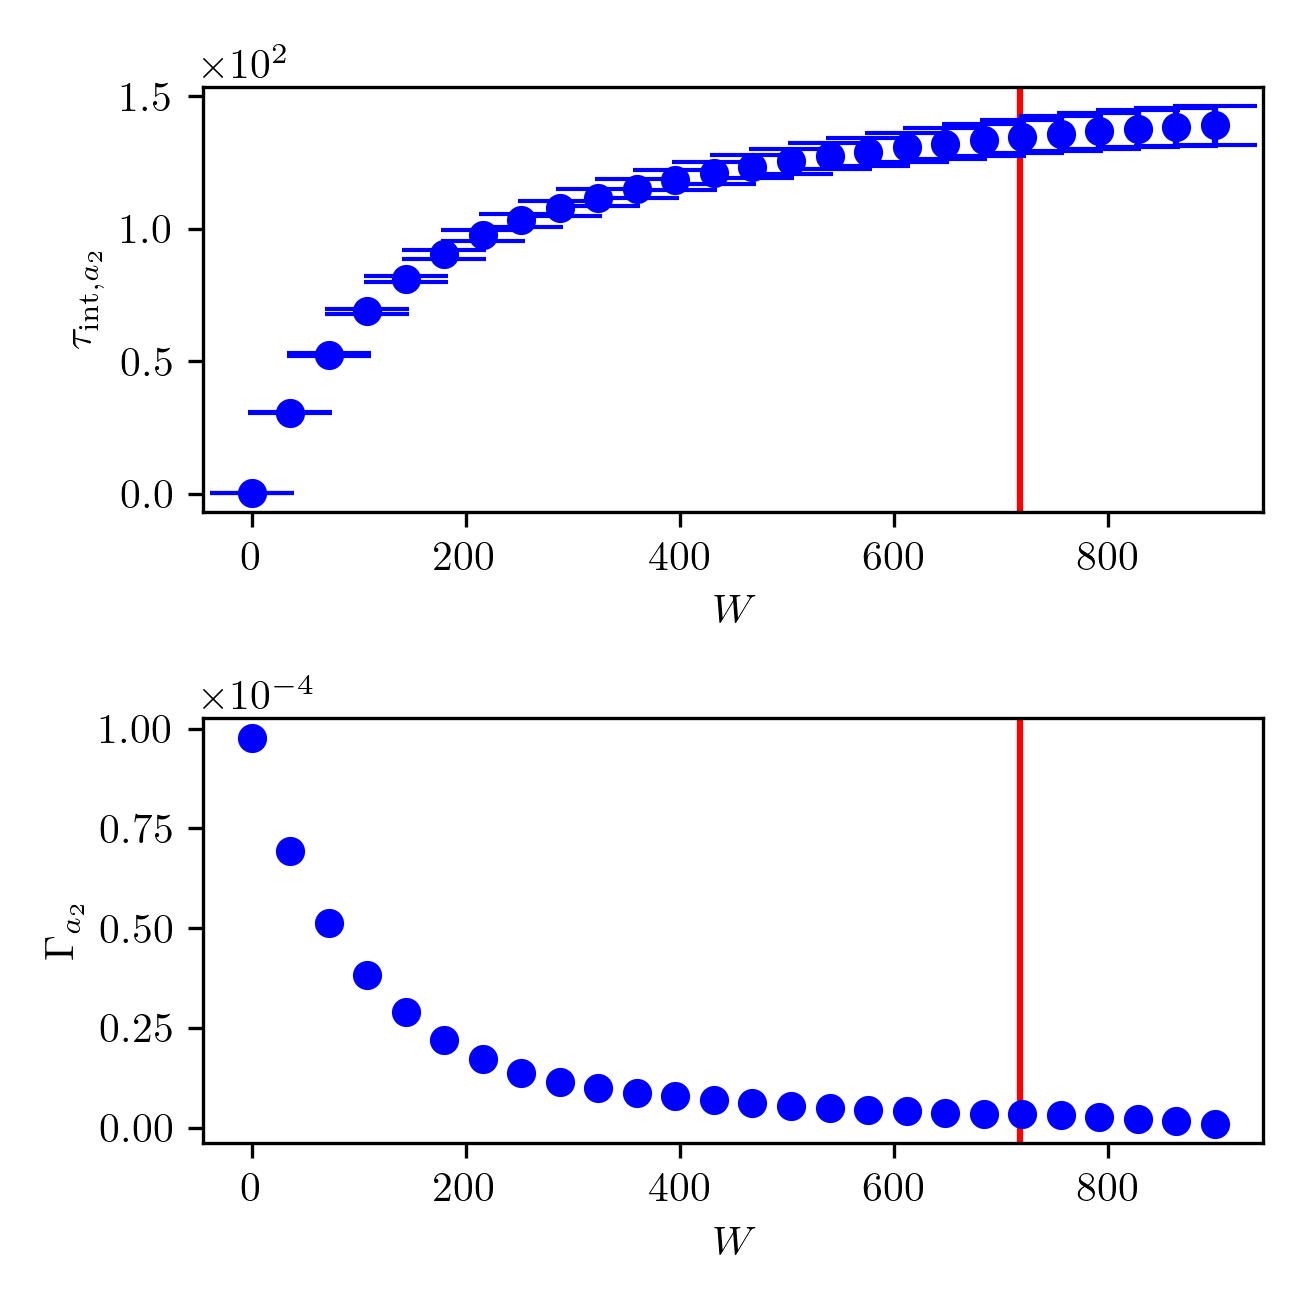
\includegraphics{UwerrTauIntTWalk10.png}
	\caption[IACT and autocorrelation function for $a_4 $ samples.]{IACT and autocorrelation function for samples $a_4 \sim \pi( \cdot | h_1, h_2,h_3,h_4,h_5,h_6,a_0,a_1,a_2,a_4,a_5,a_6,T_0,b,p_0,  \bm{y})$}
	\label{fig:}
\end{figure}


\begin{figure}[ht!]
	\centering
	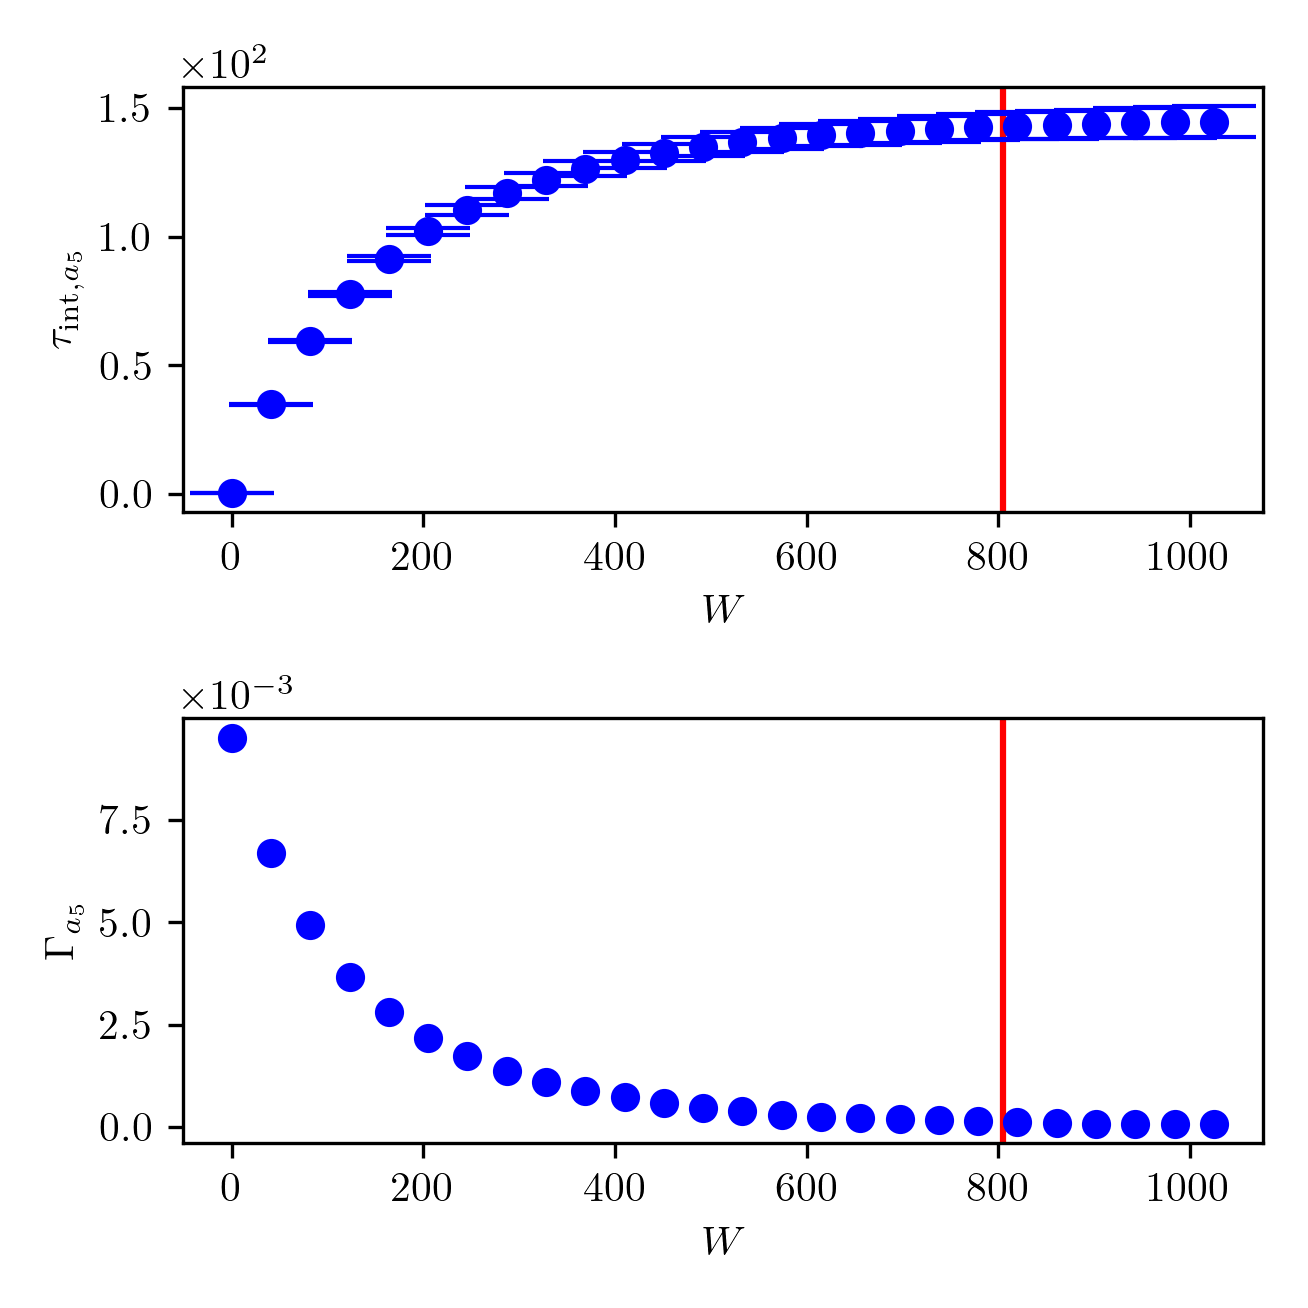
\includegraphics{UwerrTauIntTWalk11.png}
	\caption[IACT and autocorrelation function for $a_5$ samples.]{IACT and autocorrelation function for samples $a_5 \sim \pi( \cdot | h_1, h_2,h_3,h_4,h_5,h_6,a_0,a_1,a_2,a_3,a_4,a_5,T_0,b,p_0,  \bm{y})$}
	\label{fig:}
\end{figure}
\begin{figure}[ht!]
	\centering
	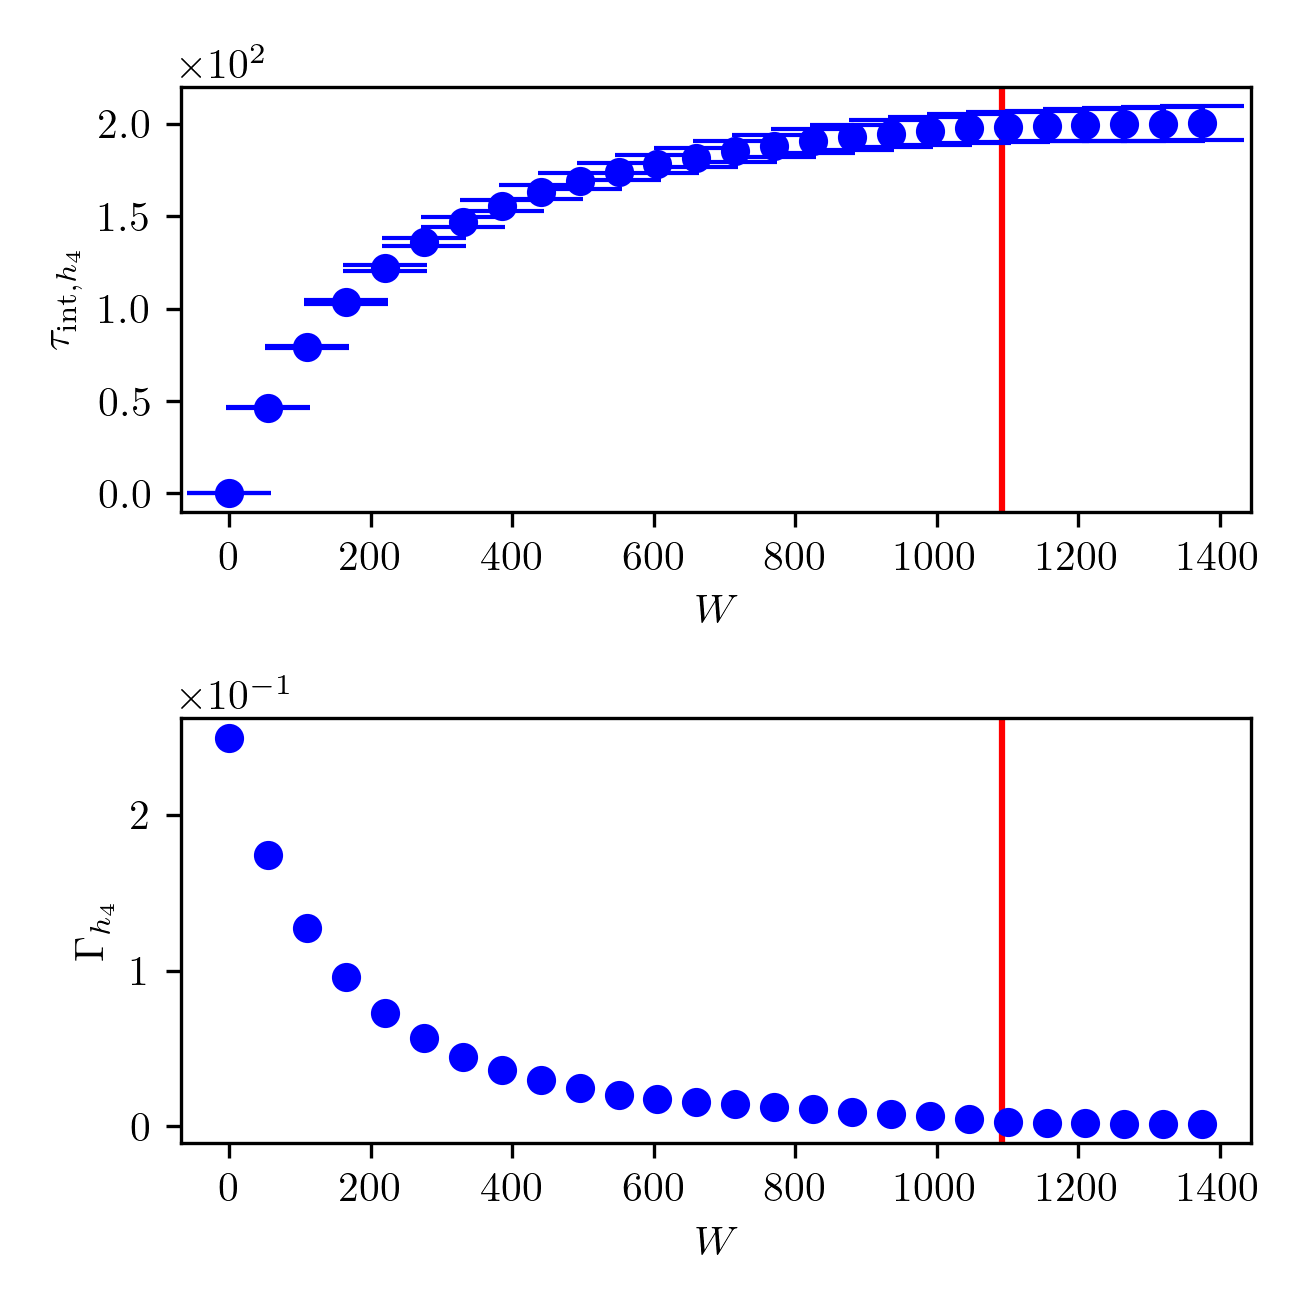
\includegraphics{UwerrTauIntTWalk12.png}
	\caption[IACT and autocorrelation function for $a_6$ samples.]{IACT and autocorrelation function for samples $a_6 \sim \pi( \cdot | h_1, h_2,h_3,h_4,h_5,h_6,a_0,a_1,a_2,a_3,a_4,a_5,T_0,b,p_0,  \bm{y})$}
	\label{fig:}
\end{figure}
\begin{figure}[ht!]
	\centering
	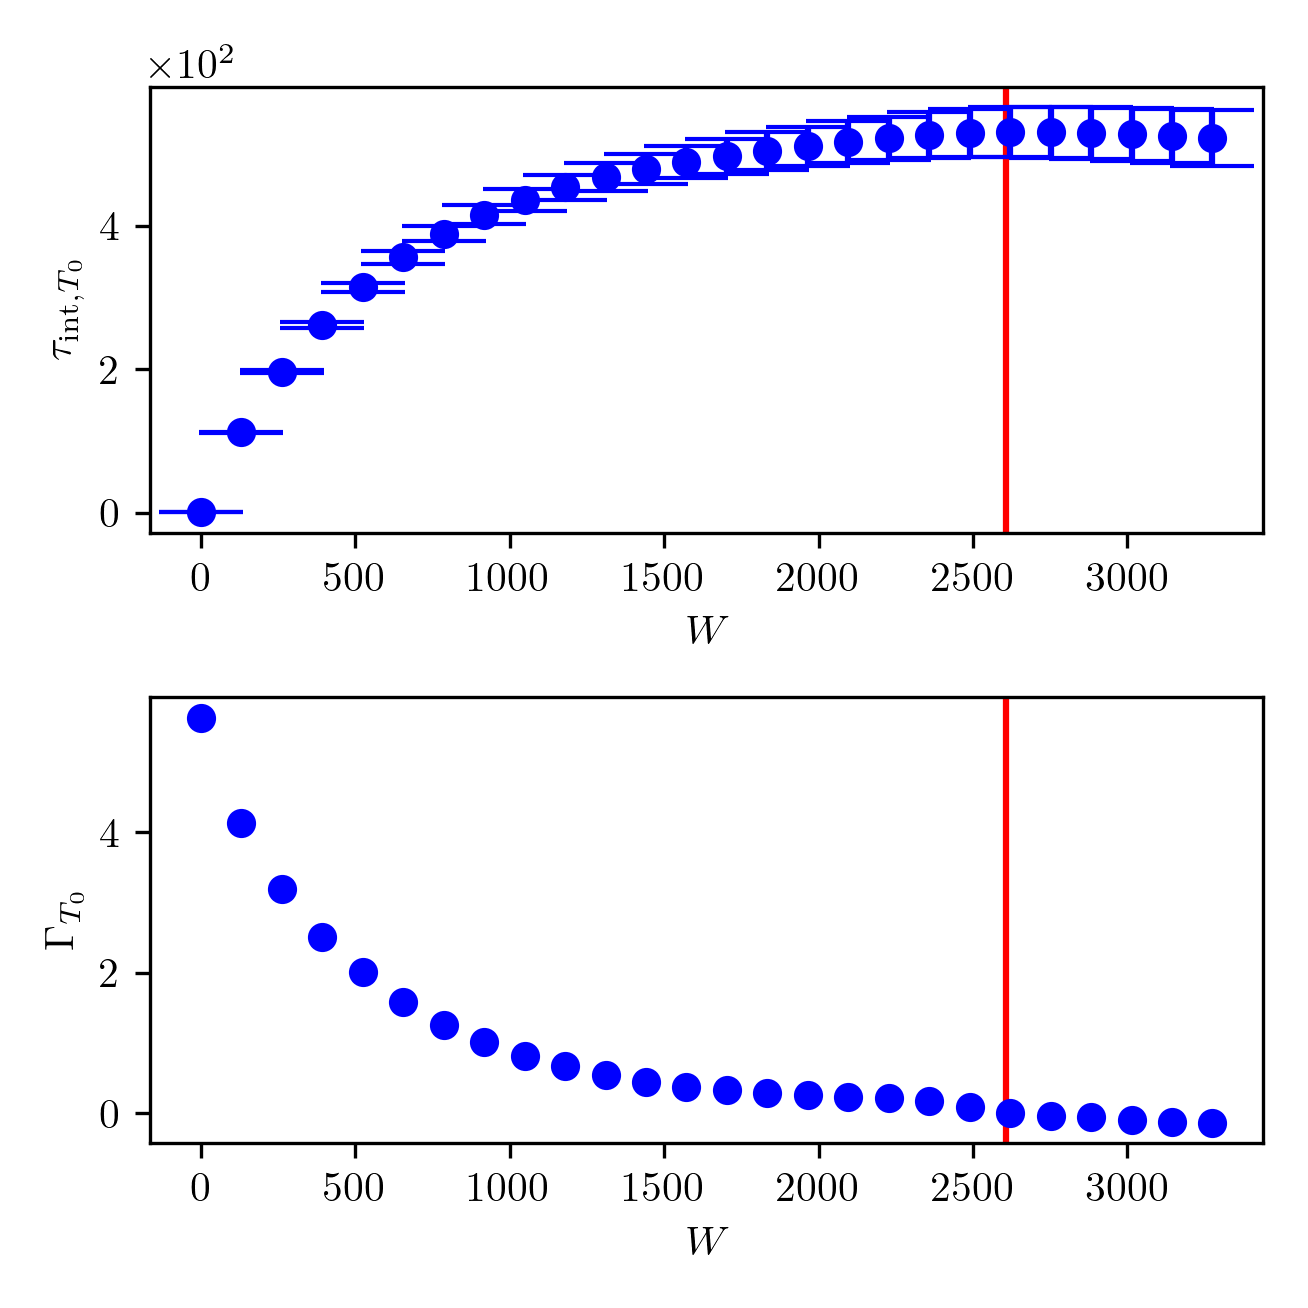
\includegraphics{UwerrTauIntTWalk13.png}
	\caption[IACT and autocorrelation function for $T_0$ samples.]{IACT and autocorrelation function for samples $T_0 \sim \pi( \cdot | h_1, h_2,h_3,h_4,h_5,h_6,a_0,a_1,a_2,a_3,a_4,a_5,a_6,b,p_0,  \bm{y})$}
	\label{fig:}
\end{figure}
\begin{figure}[ht!]
	\centering
	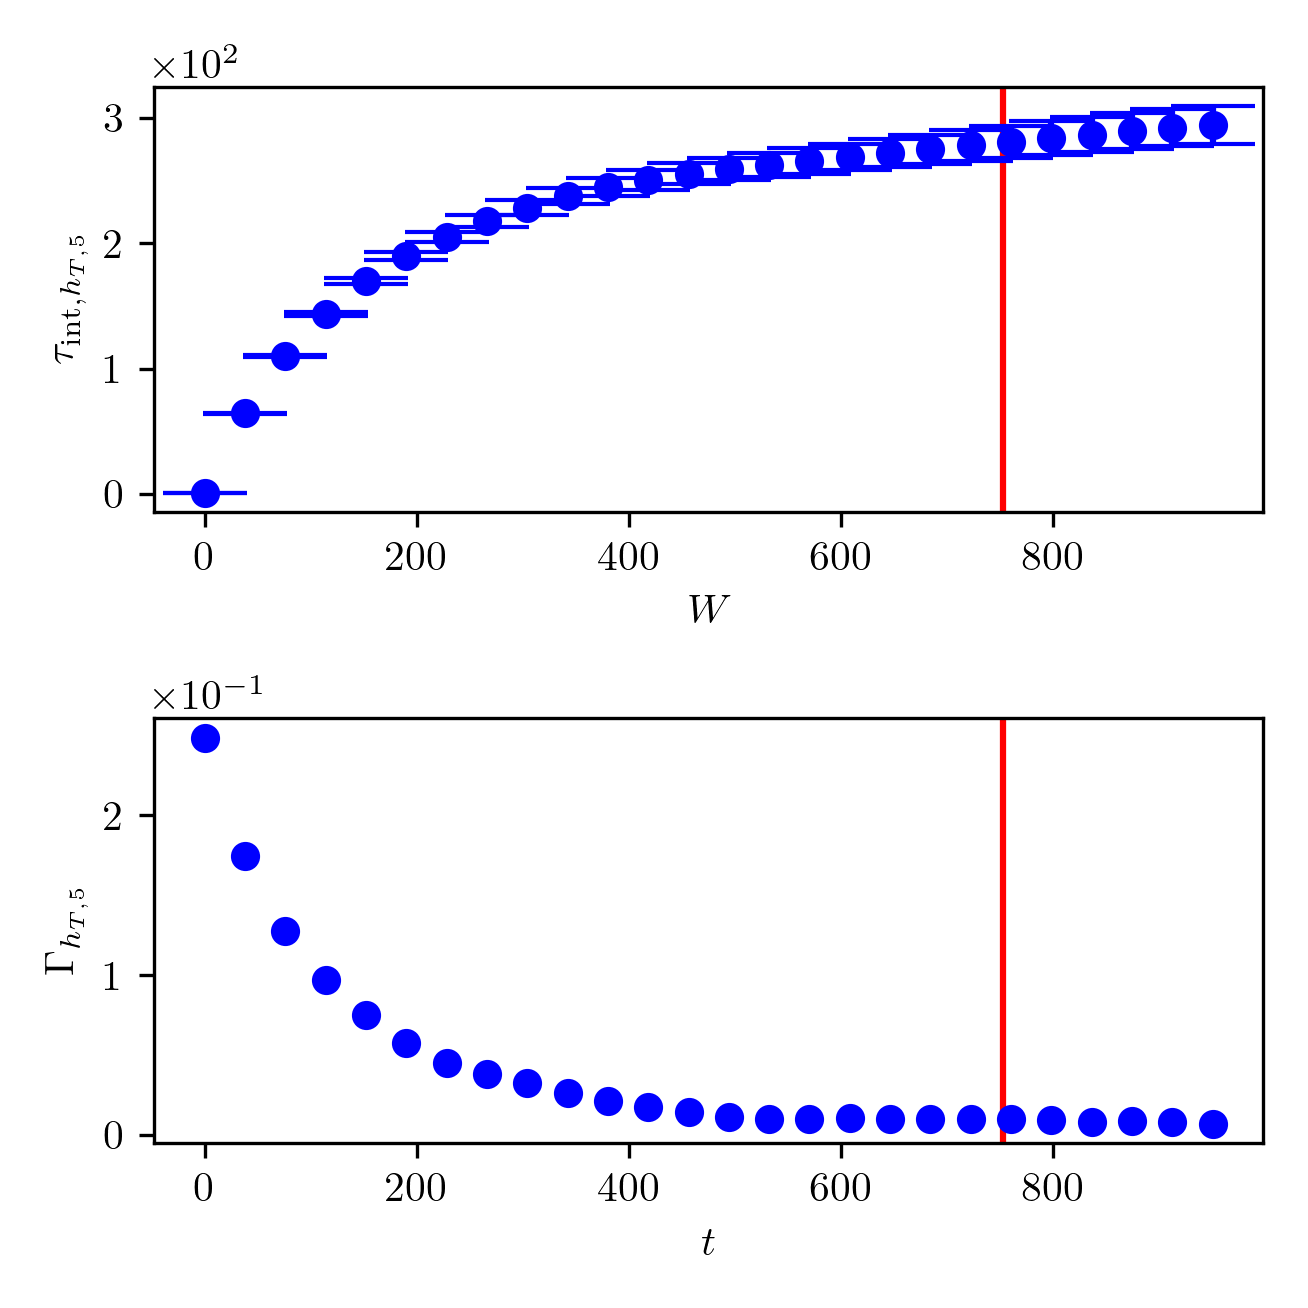
\includegraphics{UwerrTauIntTWalk14.png}
	\caption[IACT and autocorrelation function for $b$ samples.]{IACT and autocorrelation function for samples $b \sim \pi( \cdot | h_1, h_2,h_3,h_4,h_5,h_6,a_0,a_1,a_2,a_3,a_4,a_5,a_6,T_0,p_0,  \bm{y})$}
	\label{fig:}
\end{figure}

\begin{figure}[ht!]
	\centering
	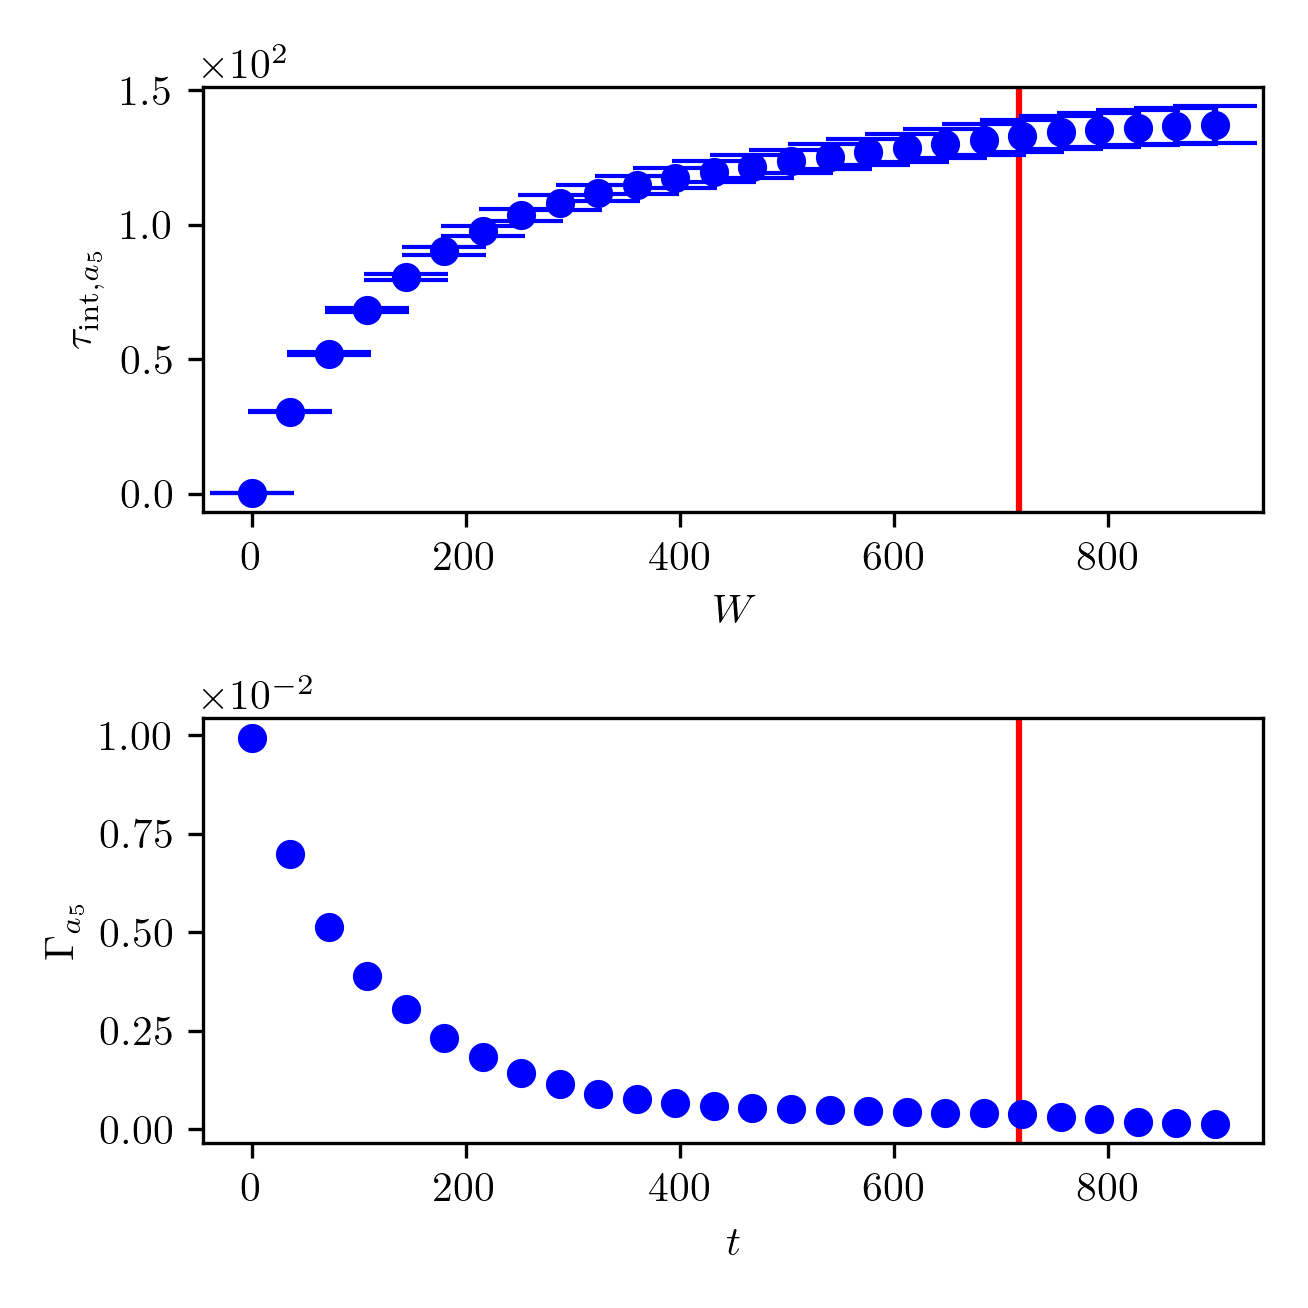
\includegraphics{UwerrTauIntTWalk15.png}
	\caption[IACT and autocorrelation function for $p_0$ samples]{IACT and autocorrelation function for samples $p_0 \sim \pi( \cdot | h_1,h_2,h_4,h_5,h_6,a_0,a_1,a_2,a_3,a_4,a_5,a_6,T_0,b, \bm{y})$}
	\label{fig:}
\end{figure}




